%% This is a sample file demonstrating the use of IJCAS.cls,
%% which is for the IJCAS (International Journal of Control, Automation, and Systems).
%%
%% 2004/03/08 by Karnes Kim
%% 2011/07/26 by CDSL, SNU
%%
%% Support sites: http://www.ijcas.com
%%
%% This code is offered as-is - no warranty - user assumes all risk.
%% Free to use, distribute and modify.
%%

%% The IJCAS class supports two column page basically. 
%%So, you need not use two column option or command.
\documentclass{IJCAS}

%% include the useful LaTeX packages:
\usepackage[hyphens]{url}  % Allows line breaks at hyphens
\usepackage[colorlinks]{hyperref}
\usepackage{array,tabularx}
\usepackage{multicol} 
\usepackage{multirow}
\usepackage{subcaption}
\usepackage{empheq}
\usepackage{enumitem}
\usepackage{tikz}

%%%% Editorial Information
%% Authors do not have to modify this section.
\journalvolumn{VV}
\journalnumber{X}
\journalyear{YYYY}
\setarticlestartpagenumber{1}
%%%% End of Editorial Information

%The environment for theorem, lemma, remark, corollary, proposition, and definition are already defined.


%The following command is needed for line break of long equations.
\allowdisplaybreaks

\newcommand{\critnum}[1]{\tikz[baseline=(char.base)]{
            \node[shape=circle,draw,inner sep=1pt](char){\textbf{#1}};}}

\newcommand{\getErrorResult}[5]{\csname#1#2#3#4#5\endcsname}


\begin{document}

\newcommand{\FlatodometryControllerVelerrorEstimateNormMeanabs}{0.034}
\newcommand{\FlatodometryControllerVelerrorEstimateNormStd}{0.033}
\newcommand{\FlatodometryControllerVelerrorEstimateXyMeanabs}{0.030}
\newcommand{\FlatodometryControllerVelerrorEstimateXyStd}{0.030}
\newcommand{\FlatodometryControllerVelerrorEstimateZMeanabs}{0.013}
\newcommand{\FlatodometryControllerVelerrorEstimateZStd}{0.021}
\newcommand{\FlatodometryControllerVelerrorLlveNormMeanabs}{0.034}
\newcommand{\FlatodometryControllerVelerrorLlveNormStd}{0.033}
\newcommand{\FlatodometryControllerVelerrorLlveXyMeanabs}{0.030}
\newcommand{\FlatodometryControllerVelerrorLlveXyStd}{0.030}
\newcommand{\FlatodometryControllerVelerrorLlveZMeanabs}{0.013}
\newcommand{\FlatodometryControllerVelerrorLlveZStd}{0.022}
\newcommand{\FlatodometryHartleyVelerrorEstimateNormMeanabs}{0.017}
\newcommand{\FlatodometryHartleyVelerrorEstimateNormStd}{0.015}
\newcommand{\FlatodometryHartleyVelerrorEstimateXyMeanabs}{0.015}
\newcommand{\FlatodometryHartleyVelerrorEstimateXyStd}{0.015}
\newcommand{\FlatodometryHartleyVelerrorEstimateZMeanabs}{0.006}
\newcommand{\FlatodometryHartleyVelerrorEstimateZStd}{0.009}
\newcommand{\FlatodometryHartleyVelerrorLlveNormMeanabs}{0.092}
\newcommand{\FlatodometryHartleyVelerrorLlveNormStd}{0.142}
\newcommand{\FlatodometryHartleyVelerrorLlveXyMeanabs}{0.090}
\newcommand{\FlatodometryHartleyVelerrorLlveXyStd}{0.141}
\newcommand{\FlatodometryHartleyVelerrorLlveZMeanabs}{0.011}
\newcommand{\FlatodometryHartleyVelerrorLlveZStd}{0.019}
\newcommand{\FlatodometryTiltVelerrorEstimateNormMeanabs}{0.019}
\newcommand{\FlatodometryTiltVelerrorEstimateNormStd}{0.019}
\newcommand{\FlatodometryTiltVelerrorEstimateXyMeanabs}{0.018}
\newcommand{\FlatodometryTiltVelerrorEstimateXyStd}{0.018}
\newcommand{\FlatodometryTiltVelerrorEstimateZMeanabs}{0.006}
\newcommand{\FlatodometryTiltVelerrorEstimateZStd}{0.010}
\newcommand{\FlatodometryTiltVelerrorLlveNormMeanabs}{0.044}
\newcommand{\FlatodometryTiltVelerrorLlveNormStd}{0.048}
\newcommand{\FlatodometryTiltVelerrorLlveXyMeanabs}{0.042}
\newcommand{\FlatodometryTiltVelerrorLlveXyStd}{0.047}
\newcommand{\FlatodometryTiltVelerrorLlveZMeanabs}{0.010}
\newcommand{\FlatodometryTiltVelerrorLlveZStd}{0.016}
\newcommand{\FlatodometryControllerRelerrorTiltMeanabs}{1.32}
\newcommand{\FlatodometryControllerRelerrorTiltStd}{2.06}
\newcommand{\FlatodometryControllerRelerrorTransxyMeanabs}{0.034}
\newcommand{\FlatodometryControllerRelerrorTransxyStd}{0.026}
\newcommand{\FlatodometryControllerRelerrorTranszMeanabs}{0.020}
\newcommand{\FlatodometryControllerRelerrorTranszStd}{0.045}
\newcommand{\FlatodometryControllerRelerrorYawMeanabs}{1.23}
\newcommand{\FlatodometryControllerRelerrorYawStd}{1.25}
\newcommand{\FlatodometryHartleyRelerrorTiltMeanabs}{1.00}
\newcommand{\FlatodometryHartleyRelerrorTiltStd}{1.84}
\newcommand{\FlatodometryHartleyRelerrorTransxyMeanabs}{0.046}
\newcommand{\FlatodometryHartleyRelerrorTransxyStd}{0.056}
\newcommand{\FlatodometryHartleyRelerrorTranszMeanabs}{0.026}
\newcommand{\FlatodometryHartleyRelerrorTranszStd}{0.051}
\newcommand{\FlatodometryHartleyRelerrorYawMeanabs}{0.96}
\newcommand{\FlatodometryHartleyRelerrorYawStd}{0.92}
\newcommand{\FlatodometryTiltRelerrorTiltMeanabs}{0.94}
\newcommand{\FlatodometryTiltRelerrorTiltStd}{1.97}
\newcommand{\FlatodometryTiltRelerrorTransxyMeanabs}{0.031}
\newcommand{\FlatodometryTiltRelerrorTransxyStd}{0.021}
\newcommand{\FlatodometryTiltRelerrorTranszMeanabs}{0.030}
\newcommand{\FlatodometryTiltRelerrorTranszStd}{0.046}
\newcommand{\FlatodometryTiltRelerrorYawMeanabs}{1.15}
\newcommand{\FlatodometryTiltRelerrorYawStd}{1.18}
\newcommand{\FlatodometryControllerAbserrorKoTrobobdRhpsaATiltMeanabs}{1.08}
\newcommand{\FlatodometryControllerAbserrorKoTrobobdRhpsaATiltStd}{0.43}
\newcommand{\FlatodometryControllerAbserrorKoTrobobdRhpsaATransxyMeanabs}{0.236}
\newcommand{\FlatodometryControllerAbserrorKoTrobobdRhpsaATransxyStd}{0.144}
\newcommand{\FlatodometryControllerAbserrorKoTrobobdRhpsaATranszMeanabs}{0.002}
\newcommand{\FlatodometryControllerAbserrorKoTrobobdRhpsaATranszStd}{0.003}
\newcommand{\FlatodometryControllerAbserrorKoTrobobdRhpsaAYawMeanabs}{2.71}
\newcommand{\FlatodometryControllerAbserrorKoTrobobdRhpsaAYawStd}{3.39}
\newcommand{\FlatodometryHartleyAbserrorKoTrobobdRhpsaATiltMeanabs}{1.22}
\newcommand{\FlatodometryHartleyAbserrorKoTrobobdRhpsaATiltStd}{0.40}
\newcommand{\FlatodometryHartleyAbserrorKoTrobobdRhpsaATransxyMeanabs}{0.260}
\newcommand{\FlatodometryHartleyAbserrorKoTrobobdRhpsaATransxyStd}{0.115}
\newcommand{\FlatodometryHartleyAbserrorKoTrobobdRhpsaATranszMeanabs}{0.160}
\newcommand{\FlatodometryHartleyAbserrorKoTrobobdRhpsaATranszStd}{0.178}
\newcommand{\FlatodometryHartleyAbserrorKoTrobobdRhpsaAYawMeanabs}{5.54}
\newcommand{\FlatodometryHartleyAbserrorKoTrobobdRhpsaAYawStd}{6.12}
\newcommand{\FlatodometryTiltAbserrorKoTrobobdRhpsaATiltMeanabs}{0.96}
\newcommand{\FlatodometryTiltAbserrorKoTrobobdRhpsaATiltStd}{0.31}
\newcommand{\FlatodometryTiltAbserrorKoTrobobdRhpsaATransxyMeanabs}{0.226}
\newcommand{\FlatodometryTiltAbserrorKoTrobobdRhpsaATransxyStd}{0.128}
\newcommand{\FlatodometryTiltAbserrorKoTrobobdRhpsaATranszMeanabs}{0.225}
\newcommand{\FlatodometryTiltAbserrorKoTrobobdRhpsaATranszStd}{0.253}
\newcommand{\FlatodometryTiltAbserrorKoTrobobdRhpsaAYawMeanabs}{2.52}
\newcommand{\FlatodometryTiltAbserrorKoTrobobdRhpsaAYawStd}{3.08}
\newcommand{\FlatodometryControllerAbserrorKoTrobobdRhpsaBTiltMeanabs}{0.90}
\newcommand{\FlatodometryControllerAbserrorKoTrobobdRhpsaBTiltStd}{0.46}
\newcommand{\FlatodometryControllerAbserrorKoTrobobdRhpsaBTransxyMeanabs}{0.179}
\newcommand{\FlatodometryControllerAbserrorKoTrobobdRhpsaBTransxyStd}{0.107}
\newcommand{\FlatodometryControllerAbserrorKoTrobobdRhpsaBTranszMeanabs}{0.002}
\newcommand{\FlatodometryControllerAbserrorKoTrobobdRhpsaBTranszStd}{0.003}
\newcommand{\FlatodometryControllerAbserrorKoTrobobdRhpsaBYawMeanabs}{2.28}
\newcommand{\FlatodometryControllerAbserrorKoTrobobdRhpsaBYawStd}{3.40}
\newcommand{\FlatodometryHartleyAbserrorKoTrobobdRhpsaBTiltMeanabs}{1.11}
\newcommand{\FlatodometryHartleyAbserrorKoTrobobdRhpsaBTiltStd}{0.36}
\newcommand{\FlatodometryHartleyAbserrorKoTrobobdRhpsaBTransxyMeanabs}{0.154}
\newcommand{\FlatodometryHartleyAbserrorKoTrobobdRhpsaBTransxyStd}{0.100}
\newcommand{\FlatodometryHartleyAbserrorKoTrobobdRhpsaBTranszMeanabs}{0.154}
\newcommand{\FlatodometryHartleyAbserrorKoTrobobdRhpsaBTranszStd}{0.177}
\newcommand{\FlatodometryHartleyAbserrorKoTrobobdRhpsaBYawMeanabs}{2.05}
\newcommand{\FlatodometryHartleyAbserrorKoTrobobdRhpsaBYawStd}{1.73}
\newcommand{\FlatodometryTiltAbserrorKoTrobobdRhpsaBTiltMeanabs}{0.84}
\newcommand{\FlatodometryTiltAbserrorKoTrobobdRhpsaBTiltStd}{0.30}
\newcommand{\FlatodometryTiltAbserrorKoTrobobdRhpsaBTransxyMeanabs}{0.168}
\newcommand{\FlatodometryTiltAbserrorKoTrobobdRhpsaBTransxyStd}{0.101}
\newcommand{\FlatodometryTiltAbserrorKoTrobobdRhpsaBTranszMeanabs}{0.196}
\newcommand{\FlatodometryTiltAbserrorKoTrobobdRhpsaBTranszStd}{0.228}
\newcommand{\FlatodometryTiltAbserrorKoTrobobdRhpsaBYawMeanabs}{4.18}
\newcommand{\FlatodometryTiltAbserrorKoTrobobdRhpsaBYawStd}{4.88}
\newcommand{\FlatodometryControllerAbserrorKoTrobobdRhpsaCTiltMeanabs}{1.04}
\newcommand{\FlatodometryControllerAbserrorKoTrobobdRhpsaCTiltStd}{0.48}
\newcommand{\FlatodometryControllerAbserrorKoTrobobdRhpsaCTransxyMeanabs}{0.303}
\newcommand{\FlatodometryControllerAbserrorKoTrobobdRhpsaCTransxyStd}{0.189}
\newcommand{\FlatodometryControllerAbserrorKoTrobobdRhpsaCTranszMeanabs}{0.002}
\newcommand{\FlatodometryControllerAbserrorKoTrobobdRhpsaCTranszStd}{0.003}
\newcommand{\FlatodometryControllerAbserrorKoTrobobdRhpsaCYawMeanabs}{4.72}
\newcommand{\FlatodometryControllerAbserrorKoTrobobdRhpsaCYawStd}{5.31}
\newcommand{\FlatodometryHartleyAbserrorKoTrobobdRhpsaCTiltMeanabs}{1.01}
\newcommand{\FlatodometryHartleyAbserrorKoTrobobdRhpsaCTiltStd}{0.36}
\newcommand{\FlatodometryHartleyAbserrorKoTrobobdRhpsaCTransxyMeanabs}{0.155}
\newcommand{\FlatodometryHartleyAbserrorKoTrobobdRhpsaCTransxyStd}{0.112}
\newcommand{\FlatodometryHartleyAbserrorKoTrobobdRhpsaCTranszMeanabs}{0.150}
\newcommand{\FlatodometryHartleyAbserrorKoTrobobdRhpsaCTranszStd}{0.165}
\newcommand{\FlatodometryHartleyAbserrorKoTrobobdRhpsaCYawMeanabs}{3.05}
\newcommand{\FlatodometryHartleyAbserrorKoTrobobdRhpsaCYawStd}{3.30}
\newcommand{\FlatodometryTiltAbserrorKoTrobobdRhpsaCTiltMeanabs}{0.76}
\newcommand{\FlatodometryTiltAbserrorKoTrobobdRhpsaCTiltStd}{0.32}
\newcommand{\FlatodometryTiltAbserrorKoTrobobdRhpsaCTransxyMeanabs}{0.203}
\newcommand{\FlatodometryTiltAbserrorKoTrobobdRhpsaCTransxyStd}{0.104}
\newcommand{\FlatodometryTiltAbserrorKoTrobobdRhpsaCTranszMeanabs}{0.191}
\newcommand{\FlatodometryTiltAbserrorKoTrobobdRhpsaCTranszStd}{0.214}
\newcommand{\FlatodometryTiltAbserrorKoTrobobdRhpsaCYawMeanabs}{3.19}
\newcommand{\FlatodometryTiltAbserrorKoTrobobdRhpsaCYawStd}{3.78}
\newcommand{\FlatodometryControllerAbserrorKoTrobobdRhpsaDTiltMeanabs}{14.36}
\newcommand{\FlatodometryControllerAbserrorKoTrobobdRhpsaDTiltStd}{0.61}
\newcommand{\FlatodometryControllerAbserrorKoTrobobdRhpsaDTransxyMeanabs}{0.401}
\newcommand{\FlatodometryControllerAbserrorKoTrobobdRhpsaDTransxyStd}{0.367}
\newcommand{\FlatodometryControllerAbserrorKoTrobobdRhpsaDTranszMeanabs}{0.002}
\newcommand{\FlatodometryControllerAbserrorKoTrobobdRhpsaDTranszStd}{0.003}
\newcommand{\FlatodometryControllerAbserrorKoTrobobdRhpsaDYawMeanabs}{5.59}
\newcommand{\FlatodometryControllerAbserrorKoTrobobdRhpsaDYawStd}{7.47}
\newcommand{\FlatodometryHartleyAbserrorKoTrobobdRhpsaDTiltMeanabs}{13.18}
\newcommand{\FlatodometryHartleyAbserrorKoTrobobdRhpsaDTiltStd}{0.53}
\newcommand{\FlatodometryHartleyAbserrorKoTrobobdRhpsaDTransxyMeanabs}{0.300}
\newcommand{\FlatodometryHartleyAbserrorKoTrobobdRhpsaDTransxyStd}{0.256}
\newcommand{\FlatodometryHartleyAbserrorKoTrobobdRhpsaDTranszMeanabs}{0.162}
\newcommand{\FlatodometryHartleyAbserrorKoTrobobdRhpsaDTranszStd}{0.183}
\newcommand{\FlatodometryHartleyAbserrorKoTrobobdRhpsaDYawMeanabs}{11.91}
\newcommand{\FlatodometryHartleyAbserrorKoTrobobdRhpsaDYawStd}{12.38}
\newcommand{\FlatodometryTiltAbserrorKoTrobobdRhpsaDTiltMeanabs}{13.71}
\newcommand{\FlatodometryTiltAbserrorKoTrobobdRhpsaDTiltStd}{0.26}
\newcommand{\FlatodometryTiltAbserrorKoTrobobdRhpsaDTransxyMeanabs}{0.282}
\newcommand{\FlatodometryTiltAbserrorKoTrobobdRhpsaDTransxyStd}{0.209}
\newcommand{\FlatodometryTiltAbserrorKoTrobobdRhpsaDTranszMeanabs}{0.212}
\newcommand{\FlatodometryTiltAbserrorKoTrobobdRhpsaDTranszStd}{0.243}
\newcommand{\FlatodometryTiltAbserrorKoTrobobdRhpsaDYawMeanabs}{3.62}
\newcommand{\FlatodometryTiltAbserrorKoTrobobdRhpsaDYawStd}{4.01}
\newcommand{\FlatodometryControllerAbserrorKoTrobobdRhpsaETiltMeanabs}{1.82}
\newcommand{\FlatodometryControllerAbserrorKoTrobobdRhpsaETiltStd}{0.52}
\newcommand{\FlatodometryControllerAbserrorKoTrobobdRhpsaETransxyMeanabs}{0.238}
\newcommand{\FlatodometryControllerAbserrorKoTrobobdRhpsaETransxyStd}{0.122}
\newcommand{\FlatodometryControllerAbserrorKoTrobobdRhpsaETranszMeanabs}{0.003}
\newcommand{\FlatodometryControllerAbserrorKoTrobobdRhpsaETranszStd}{0.003}
\newcommand{\FlatodometryControllerAbserrorKoTrobobdRhpsaEYawMeanabs}{2.77}
\newcommand{\FlatodometryControllerAbserrorKoTrobobdRhpsaEYawStd}{2.01}
\newcommand{\FlatodometryHartleyAbserrorKoTrobobdRhpsaETiltMeanabs}{0.57}
\newcommand{\FlatodometryHartleyAbserrorKoTrobobdRhpsaETiltStd}{0.46}
\newcommand{\FlatodometryHartleyAbserrorKoTrobobdRhpsaETransxyMeanabs}{0.205}
\newcommand{\FlatodometryHartleyAbserrorKoTrobobdRhpsaETransxyStd}{0.104}
\newcommand{\FlatodometryHartleyAbserrorKoTrobobdRhpsaETranszMeanabs}{0.147}
\newcommand{\FlatodometryHartleyAbserrorKoTrobobdRhpsaETranszStd}{0.171}
\newcommand{\FlatodometryHartleyAbserrorKoTrobobdRhpsaEYawMeanabs}{4.26}
\newcommand{\FlatodometryHartleyAbserrorKoTrobobdRhpsaEYawStd}{4.55}
\newcommand{\FlatodometryTiltAbserrorKoTrobobdRhpsaETiltMeanabs}{1.21}
\newcommand{\FlatodometryTiltAbserrorKoTrobobdRhpsaETiltStd}{0.24}
\newcommand{\FlatodometryTiltAbserrorKoTrobobdRhpsaETransxyMeanabs}{0.197}
\newcommand{\FlatodometryTiltAbserrorKoTrobobdRhpsaETransxyStd}{0.092}
\newcommand{\FlatodometryTiltAbserrorKoTrobobdRhpsaETranszMeanabs}{0.203}
\newcommand{\FlatodometryTiltAbserrorKoTrobobdRhpsaETranszStd}{0.232}
\newcommand{\FlatodometryTiltAbserrorKoTrobobdRhpsaEYawMeanabs}{2.44}
\newcommand{\FlatodometryTiltAbserrorKoTrobobdRhpsaEYawStd}{2.37}



\newcommand{\MulticontactControllerVelerrorEstimateNormMeanabs}{0.034}
\newcommand{\MulticontactControllerVelerrorEstimateNormStd}{0.033}
\newcommand{\MulticontactControllerVelerrorEstimateXyMeanabs}{0.030}
\newcommand{\MulticontactControllerVelerrorEstimateXyStd}{0.030}
\newcommand{\MulticontactControllerVelerrorEstimateZMeanabs}{0.013}
\newcommand{\MulticontactControllerVelerrorEstimateZStd}{0.021}
\newcommand{\MulticontactControllerVelerrorLlveNormMeanabs}{0.034}
\newcommand{\MulticontactControllerVelerrorLlveNormStd}{0.033}
\newcommand{\MulticontactControllerVelerrorLlveXyMeanabs}{0.030}
\newcommand{\MulticontactControllerVelerrorLlveXyStd}{0.030}
\newcommand{\MulticontactControllerVelerrorLlveZMeanabs}{0.013}
\newcommand{\MulticontactControllerVelerrorLlveZStd}{0.022}
\newcommand{\MulticontactHartleyVelerrorEstimateNormMeanabs}{0.017}
\newcommand{\MulticontactHartleyVelerrorEstimateNormStd}{0.015}
\newcommand{\MulticontactHartleyVelerrorEstimateXyMeanabs}{0.015}
\newcommand{\MulticontactHartleyVelerrorEstimateXyStd}{0.015}
\newcommand{\MulticontactHartleyVelerrorEstimateZMeanabs}{0.006}
\newcommand{\MulticontactHartleyVelerrorEstimateZStd}{0.009}
\newcommand{\MulticontactHartleyVelerrorLlveNormMeanabs}{0.092}
\newcommand{\MulticontactHartleyVelerrorLlveNormStd}{0.142}
\newcommand{\MulticontactHartleyVelerrorLlveXyMeanabs}{0.090}
\newcommand{\MulticontactHartleyVelerrorLlveXyStd}{0.141}
\newcommand{\MulticontactHartleyVelerrorLlveZMeanabs}{0.011}
\newcommand{\MulticontactHartleyVelerrorLlveZStd}{0.019}
\newcommand{\MulticontactTiltVelerrorEstimateNormMeanabs}{0.019}
\newcommand{\MulticontactTiltVelerrorEstimateNormStd}{0.019}
\newcommand{\MulticontactTiltVelerrorEstimateXyMeanabs}{0.018}
\newcommand{\MulticontactTiltVelerrorEstimateXyStd}{0.018}
\newcommand{\MulticontactTiltVelerrorEstimateZMeanabs}{0.006}
\newcommand{\MulticontactTiltVelerrorEstimateZStd}{0.010}
\newcommand{\MulticontactTiltVelerrorLlveNormMeanabs}{0.044}
\newcommand{\MulticontactTiltVelerrorLlveNormStd}{0.048}
\newcommand{\MulticontactTiltVelerrorLlveXyMeanabs}{0.042}
\newcommand{\MulticontactTiltVelerrorLlveXyStd}{0.047}
\newcommand{\MulticontactTiltVelerrorLlveZMeanabs}{0.010}
\newcommand{\MulticontactTiltVelerrorLlveZStd}{0.016}
\newcommand{\MulticontactControllerRelerrorTiltMeanabs}{1.16}
\newcommand{\MulticontactControllerRelerrorTiltStd}{0.58}
\newcommand{\MulticontactControllerRelerrorTransxyMeanabs}{0.016}
\newcommand{\MulticontactControllerRelerrorTransxyStd}{0.008}
\newcommand{\MulticontactControllerRelerrorTranszMeanabs}{0.006}
\newcommand{\MulticontactControllerRelerrorTranszStd}{0.007}
\newcommand{\MulticontactControllerRelerrorYawMeanabs}{0.50}
\newcommand{\MulticontactControllerRelerrorYawStd}{0.35}
\newcommand{\MulticontactHartleyRelerrorTiltMeanabs}{0.57}
\newcommand{\MulticontactHartleyRelerrorTiltStd}{1.02}
\newcommand{\MulticontactHartleyRelerrorTransxyMeanabs}{0.012}
\newcommand{\MulticontactHartleyRelerrorTransxyStd}{0.016}
\newcommand{\MulticontactHartleyRelerrorTranszMeanabs}{0.004}
\newcommand{\MulticontactHartleyRelerrorTranszStd}{0.007}
\newcommand{\MulticontactHartleyRelerrorYawMeanabs}{0.47}
\newcommand{\MulticontactHartleyRelerrorYawStd}{0.65}
\newcommand{\MulticontactTiltRelerrorTiltMeanabs}{0.23}
\newcommand{\MulticontactTiltRelerrorTiltStd}{0.17}
\newcommand{\MulticontactTiltRelerrorTransxyMeanabs}{0.007}
\newcommand{\MulticontactTiltRelerrorTransxyStd}{0.005}
\newcommand{\MulticontactTiltRelerrorTranszMeanabs}{0.002}
\newcommand{\MulticontactTiltRelerrorTranszStd}{0.003}
\newcommand{\MulticontactTiltRelerrorYawMeanabs}{0.40}
\newcommand{\MulticontactTiltRelerrorYawStd}{0.32}
\newcommand{\MulticontactControllerAbserrorHrpeMulticontactATiltMeanabs}{0.99}
\newcommand{\MulticontactControllerAbserrorHrpeMulticontactATiltStd}{0.67}
\newcommand{\MulticontactControllerAbserrorHrpeMulticontactATransxyMeanabs}{0.019}
\newcommand{\MulticontactControllerAbserrorHrpeMulticontactATransxyStd}{0.008}
\newcommand{\MulticontactControllerAbserrorHrpeMulticontactATranszMeanabs}{0.004}
\newcommand{\MulticontactControllerAbserrorHrpeMulticontactATranszStd}{0.005}
\newcommand{\MulticontactControllerAbserrorHrpeMulticontactAYawMeanabs}{1.36}
\newcommand{\MulticontactControllerAbserrorHrpeMulticontactAYawStd}{0.74}
\newcommand{\MulticontactHartleyAbserrorHrpeMulticontactATiltMeanabs}{0.68}
\newcommand{\MulticontactHartleyAbserrorHrpeMulticontactATiltStd}{0.26}
\newcommand{\MulticontactHartleyAbserrorHrpeMulticontactATransxyMeanabs}{0.006}
\newcommand{\MulticontactHartleyAbserrorHrpeMulticontactATransxyStd}{0.003}
\newcommand{\MulticontactHartleyAbserrorHrpeMulticontactATranszMeanabs}{0.003}
\newcommand{\MulticontactHartleyAbserrorHrpeMulticontactATranszStd}{0.003}
\newcommand{\MulticontactHartleyAbserrorHrpeMulticontactAYawMeanabs}{1.35}
\newcommand{\MulticontactHartleyAbserrorHrpeMulticontactAYawStd}{0.67}
\newcommand{\MulticontactTiltAbserrorHrpeMulticontactATiltMeanabs}{0.34}
\newcommand{\MulticontactTiltAbserrorHrpeMulticontactATiltStd}{0.17}
\newcommand{\MulticontactTiltAbserrorHrpeMulticontactATransxyMeanabs}{0.009}
\newcommand{\MulticontactTiltAbserrorHrpeMulticontactATransxyStd}{0.003}
\newcommand{\MulticontactTiltAbserrorHrpeMulticontactATranszMeanabs}{0.004}
\newcommand{\MulticontactTiltAbserrorHrpeMulticontactATranszStd}{0.005}
\newcommand{\MulticontactTiltAbserrorHrpeMulticontactAYawMeanabs}{1.06}
\newcommand{\MulticontactTiltAbserrorHrpeMulticontactAYawStd}{0.93}



% the \title command
\title{{\scshape Valinor}: a Lightweight Leg Inertial Odometry for Humanoid Robots}

% the \author command
% the \orcid{orcid number}
\author{Arnaud Demont*\orcid{0009-0006-8325-8331}, Mehdi Benallegue\orcid{0000-0001-7537-9498}, Thomas Duvinage\orcid{0009-0008-9939-8237}, and Abdelaziz Benallegue\orcid{0000-0003-2316-7981}}


% the abstract environment
\begin{abstract}
This article presents {\scshape Valinor} (Velocity-Aided Leg Inertial Nonlinear Odometry and Registration), a method for lightweight yet accurate Leg-Inertial odometry for humanoid robots. {\scshape Valinor} builds upon the Tilt Observer, a complementary filter that estimates the IMU's tilt and linear velocity with strong mathematical convergence guarantees, associating it with Leg odometry. We introduce an axis-agnostic fusion method that coherently combines the Tilt Observer's tilt estimate with the Leg odometry's yaw. We argue that this method is less arbitrary and more mathematically sound than those based on other orientation representations, especially on Euler angles.
We validate {\scshape Valinor} on real-world experiments with two humanoid robots. Results show that, while being 7.5 times faster than the state-of-the-art method used for comparison, {\scshape Valinor} achieves estimation performance on par with it. This makes {\scshape Valinor} a strong candidate for feedback in balance control, as well as for task planning and execution within the robot's local workspace. 
Beyond this contribution, we hope to highlight the broader need for estimation methods that are not only accurate and efficient, but also grounded in strong mathematical guarantees, towards their safe deployment around humans.
\end{abstract}

\begin{keywords}
  Lightweight state estimation, Humanoid robots, Proprioceptive odometry, Tilt estimation, Balancing.
\end{keywords}

\maketitle


\makeAuthorInformation{
Arnaud Demont is with the CNRS-AIST JRL (Joint Robotics Laboratory), IRL, National Institute of Advanced Industrial Science and Technology (AIST), Tsukuba, Ibaraki 305-8560 Japan, Université Paris-Saclay, 91190 Gif-sur-Yvette, France, and Laboratoire d'Ingénierie des Systèmes de Versailles, 78140 Vélizy, France (email: arnaud.demont@aist.go.jp). 
Mehdi Benallegue and Thomas Duvinage are with the CNRS-AIST JRL (Joint Robotics Laboratory), IRL, National Institute of Advanced Industrial Science and Technology (AIST), Tsukuba, Ibaraki 305-8560 Japan (emails: mehdi.benallegue@aist.go.jp, thomas.duvinage@aist.go.jp).
Abdelaziz Benallegue is with the CNRS-AIST JRL (Joint Robotics Laboratory), IRL, National Institute of Advanced Industrial Science and Technology (AIST), Tsukuba, Ibaraki 305-8560 Japan, and Laboratoire d'Ingénierie des Systèmes de Versailles, 78140 Vélizy, France (email: abdelaziz.benallegue@uvsq.fr). 

* Corresponding author.
}

\runningtitle{2025}{Arnaud Demont, Mehdi Benallegue, Thomas Duvinage and Abdelaziz Benallegue}{Manuscript Template for the International Journal of Control, Automation, and Systems: ICROS {\&} KIEE}{xxx}{xxxx}{x}


\section{INTRODUCTION}


Humanoid robot navigation in real-world environments remains a core challenge in robotics. For robots to be deployed at scale in society and industry, whether in healthcare facilities or warehouses, they must operate robustly in dynamic, unstructured, and human-centric environments~\cite{Kuindersma2015OptimizationBasedLocomAtlas}. This requires strong guarantees on their ability to plan motion, and execute actions in real time. In comparison to other legged robots, the control of humanoids is particularly difficult due to their complex underactuated dynamics controlled through contact with the environment~\cite{sugihara2020surveyDynamicsHumanoids}. Their control must therefore be as theoretically grounded as possible, in order to ensure safe, predictable, and certifiable behavior~\cite{chlipala2013CertifiedProgrammingCoq}.

In the meantime, methods for motion generation continue to gain in complexity and capability. Notably, Model Predictive Control (MPC)~\cite{Katayama2023MpcLeggedHumanoid, Dantec2022WholeBodyMPCTorqueControl, Dallard2024AdiosStabilizers}, reinforcement learning-based controllers~\cite{Peters2003ReinforcmentLearningForHumanoid, Li2025RLVersatileDynamicRobustBipedalLocom}, and foundation models~\cite{Bjorck2025GrootN1, kawaharazuka2024RealWorldApplicationsFoundationModels} are becoming more prevalent due to their ability to handle long-horizon planning, complex dynamics, and to their versatility. However, these advances come at the cost of increased computational complexity, running them in real-time on resource-limited platforms like embedded systems thus becomes challenging~\cite{Zeilinger2014RealTimeRobustMPC, findeisen2004computationalDelayNMPC, Thodoroff2022BenchmarkingRealTimeRL, Firoozi2025FoundationModelsInRobotics}. Since the control part is getting heavier, one practical solution is to reduce the computational load of other parts of the pipeline. The state estimation part is one of the cornerstones of the pipeline, since other components depend on its output and often have to wait for it before executing, and thus cannot run in parallel. It is therefore especially critical to try and reduce the computation time of the state estimation part.

State estimation for legged robots has also known notable improvements in the past years, the main trend aiming towards improving its global accuracy by incorporating more and more advanced sensors, especially exteroceptive ones, such as cameras, LiDARs, etc.~\cite{wisth2022vilens, fallon2018AccRobLocWalkRobotsImuVisLidar, Kuang2024TightlyCoupledLidarImuUwb}. Such methods show remarkable accuracies. However, they also tend to be more and more computationally expensive (e.g. the order of the millisecond for ~\cite{Kuang2024TightlyCoupledLidarImuUwb}).

For this reason, there is still a need for lightweight state estimation methods, which rather than adding new sensors, focus on improving the estimation of key variables at high frequency using the proprioceptive sensors readily available on the robot. The most common sensors for humanoids are joint encoders, inertial measurement units (IMUs) and contact force sensors such as FSR or force/torque sensors. IMUs are able to measure angular velocities and linear accelerations, including the gravitational one. It can be used to estimate the vertical direction, which we call \emph{tilt}. This is done often under the assumption that accelerations are negligible compared to the gravitational acceleration (e.g.~\cite{mahony2008NonlinearComplementaryFiltersOnSO3}). Unfortunately, this assumption cannot hold in the case of humanoids, especially with impacts and dynamic motions, which significantly degrades the estimation. IMUs signals can also be integrated to provide estimations of the positions and orientation in which is called inertial odometry, but if done for extended periods of time this would produce fast drifts because of noise and initial estimation errors.

Both issues, high accelerations and odometry drifts can be resolved thanks to a single consideration: legged robots are connected to a stable environment through their contacts. Meaning that we consider contacts to be fixed points in the environment, which provides a partial measurement of the robot's kinematics in the world using joint encoders. This consideration only makes the tilt fully observable, however dynamic the motion is~\cite{benallegue2020LyapunovStableOrientationEstimatorHumanoids}. The anchor with the environment and the kinematic data can be used also to perform legged odometry (also called ``Leg'' odometry) using the transformations between successive contacts to rebuild the world-trajectory~\cite{Lin2005ALegConfigurationMeasSystemHexapod}. This technique can be merged with IMU data and correct for the drift~\cite{bloesch2013FusionLegKineAndImu, masuya2015DeadReckoningAnchoringPivot}. This is called leg-inertial odometry.

 Violations of slippage-free contact assumption can degrade the odometry performance~\cite{lin2021legged, maravgakis2023probabilistic}. Work has thus been done to address the problem of contact slippage, for example by discarding unreliable contacts~\cite{lin2021legged, maravgakis2023probabilistic,yoon2023InvariantSmootherDynamicContactEventInformation}, or by attempting to correct the contact reference position~\cite{bloesch2013FusionLegKineAndImu,Hartley2020RIEKF, Demont2024KineticsObserver}. Despite that, the position and yaw orientation of the robot in the world frame remain unobservable~\cite{bloesch2013FusionLegKineAndImu}. Nevertheless, the methods exploiting these contacts have proven to be more than enough in concrete use-cases when the pose needs to be reliable only locally, like for remotely controlled robots~\cite{Grandia2024DesignControlBipedalRoboticCharacter} or when task planning is also made in the robot's local environment~\cite{Tsuru2023OnlineMulticontactReplanningHumanoid}, which means that drifts due to slippage remain limited for these use-cases.

In this work we propose {\scshape Valinor} (Velocity-Aided Leg Inertial Nonlinear Odometry and Registration), a method for Leg-Inertial odometry for legged robots, which relies on a highly accurate tilt estimate provided by a nonlinear complementary filter~\cite{benallegue2020LyapunovStableOrientationEstimatorHumanoids}. This complementary filter allows for a much faster computation than the conventionally used Kalman Filter (e.g.~\cite{Hartley2020RIEKF}), and offers mathematical convergence guarantees on the tilt and linear velocity estimate, aligning with our objective of lightweight yet accurate and certifiable state estimation.
The main contributions introduced in this paper are as follows:
\begin{itemize}
  \item The proposed state estimator is 7.5 times faster than the start-of-the-art method for proprioceptive odometry, while displaying on par odometry accuracy, and even improving significantly tilt estimation.
  \item We present the axis-agnostic tilt and yaw fusion, which we show to be more mathematically sound than that based on Euler angle representations.
  \item We evaluate the proposed method on real experiments with two different humanoid robots.
  \item The code of the Tilt Observer is open source\footnote{\scriptsize \url{https://github.com/ArnaudDmt/state-observation}}, as well as a ROS wrapper\footnote{\scriptsize \url{https://github.com/ArnaudDmt/state_observation_ros.git}}.
\end{itemize}

% \noindent Figure~\ref{fig:summary} provides a summary of {\scshape Valinor}'s pipeline, highlighting the contribution of each section of this paper.
% \begin{figure*}[!ht]
% \begin{center}
% 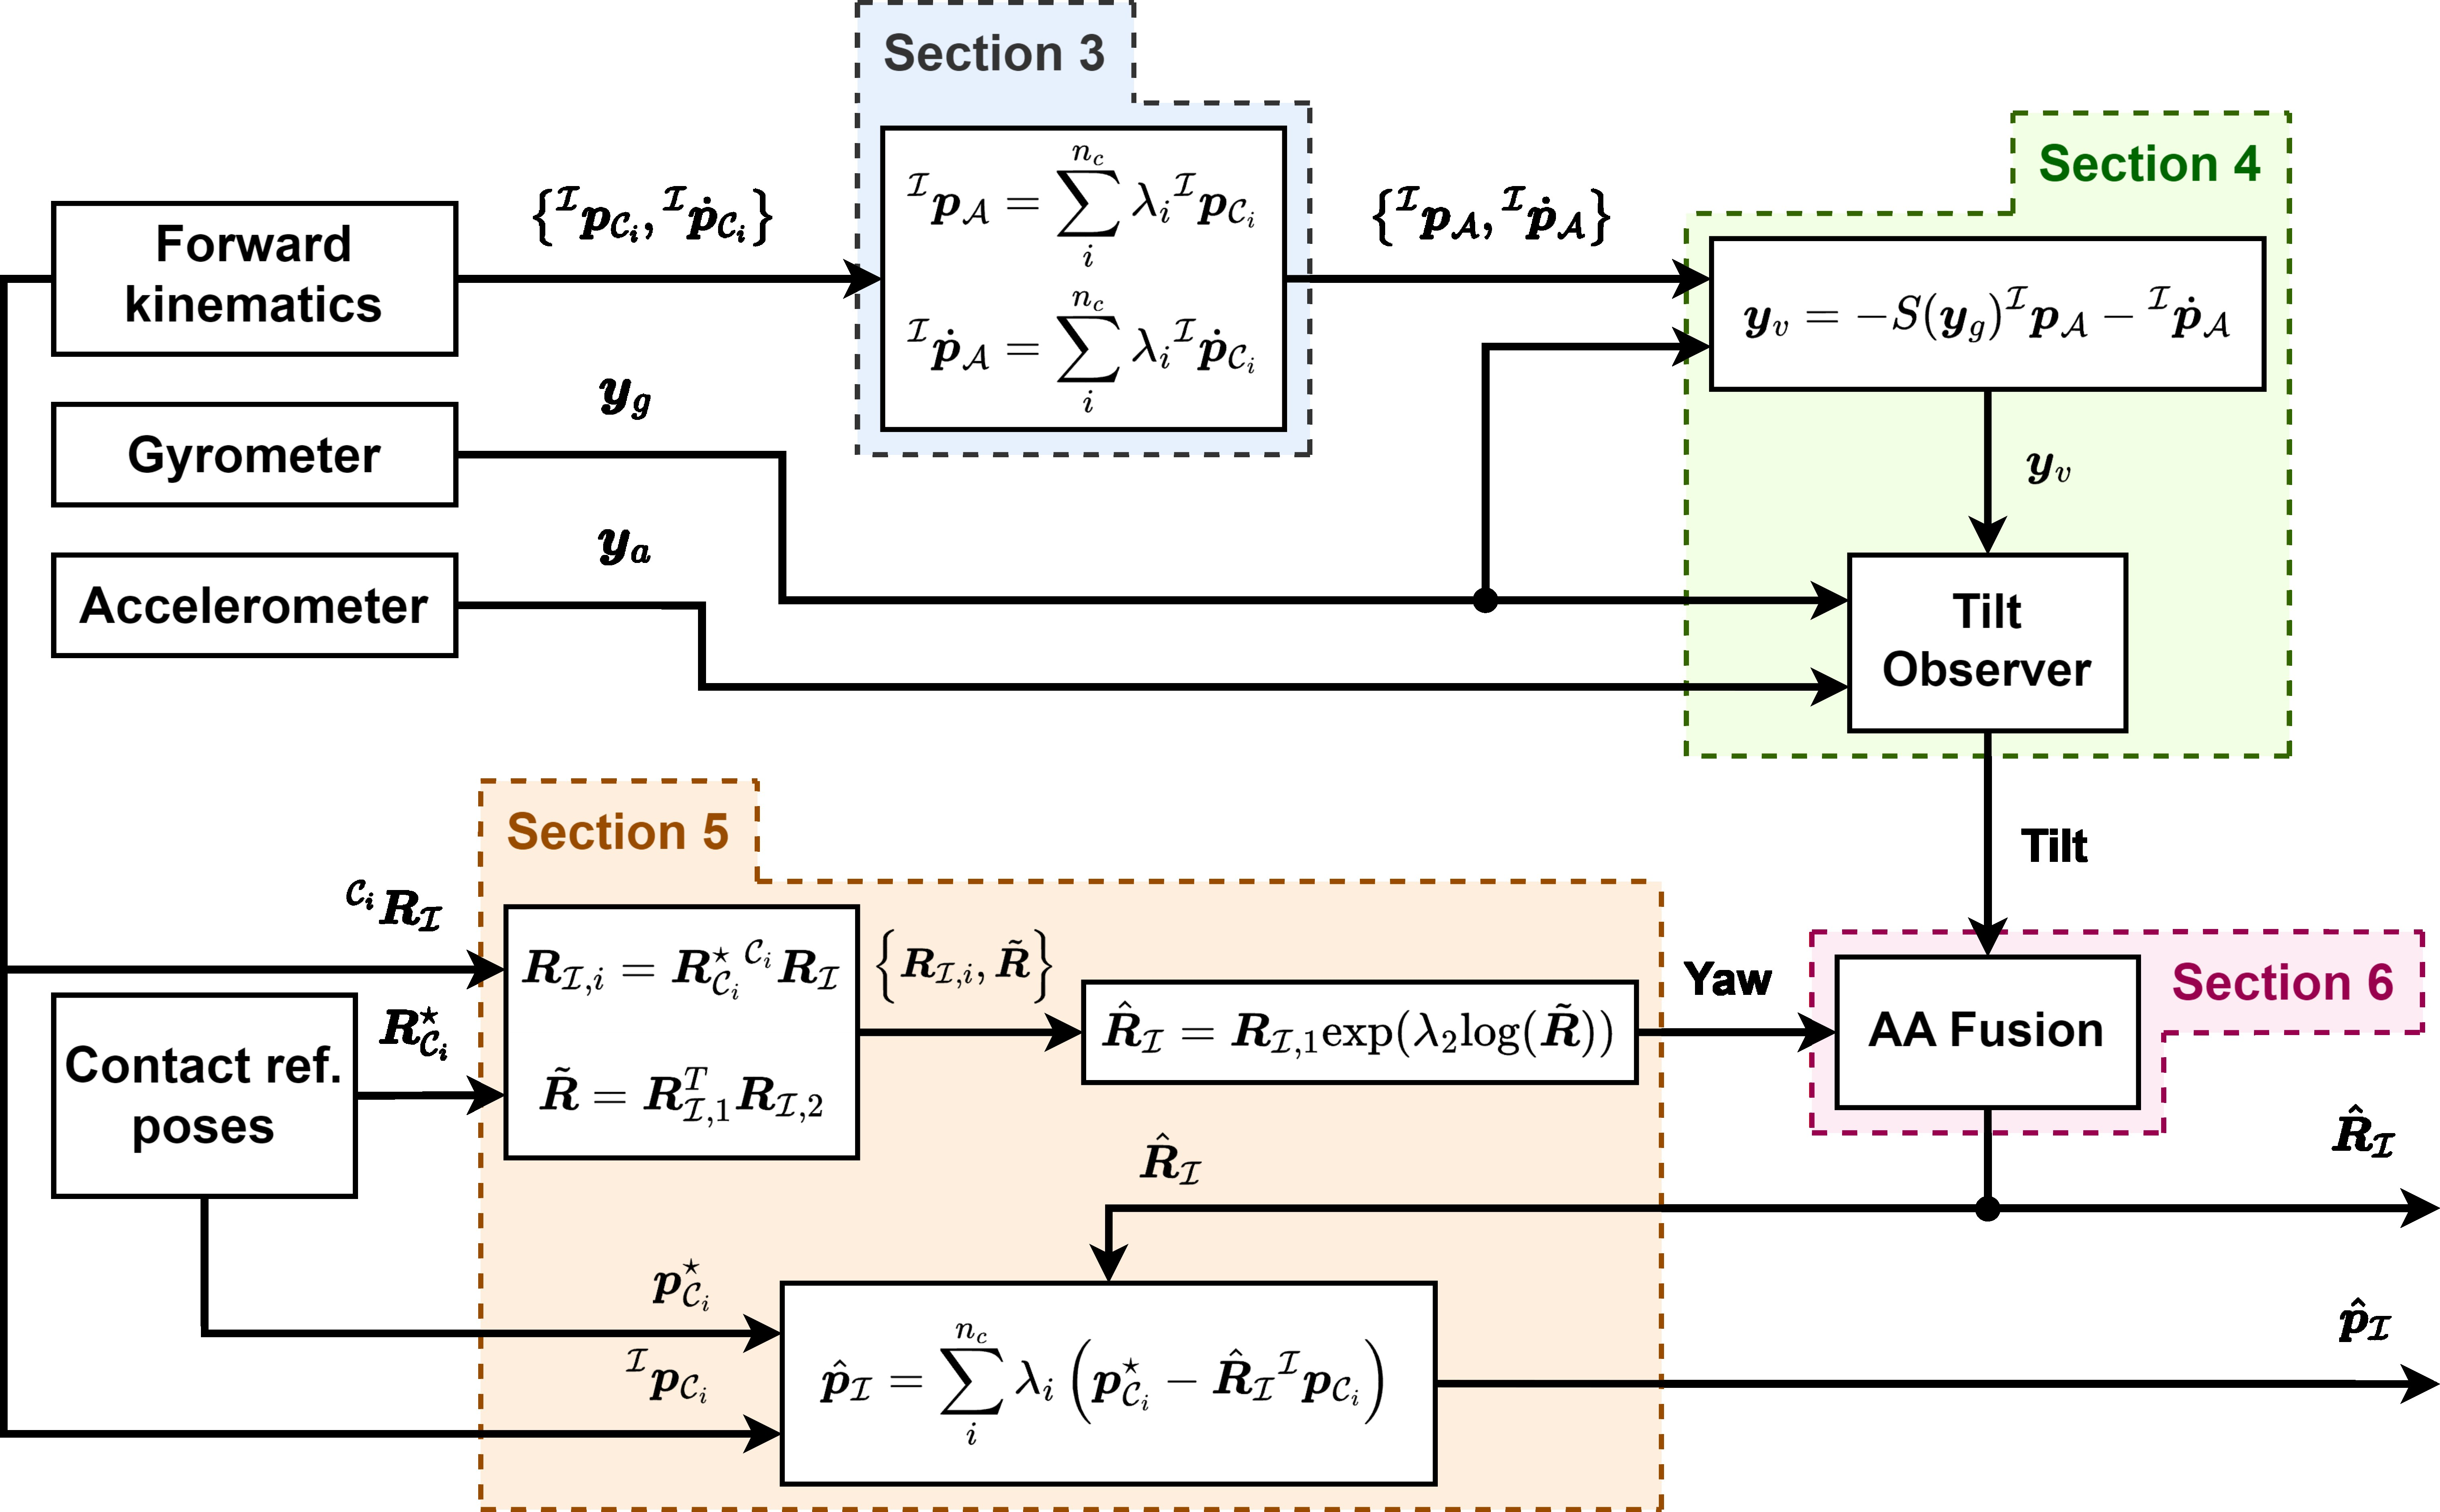
\includegraphics[width=0.6\textwidth]{summary.jpg} 
% \vskip -0.5pc
% \caption{Summary of {\scshape Valinor}'s pipeline.}\label{fig:summary}
% \end{center}
% \vskip -1.5pc
% \end{figure*}

\begin{figure*}[!ht]
    \subfloat[]{
        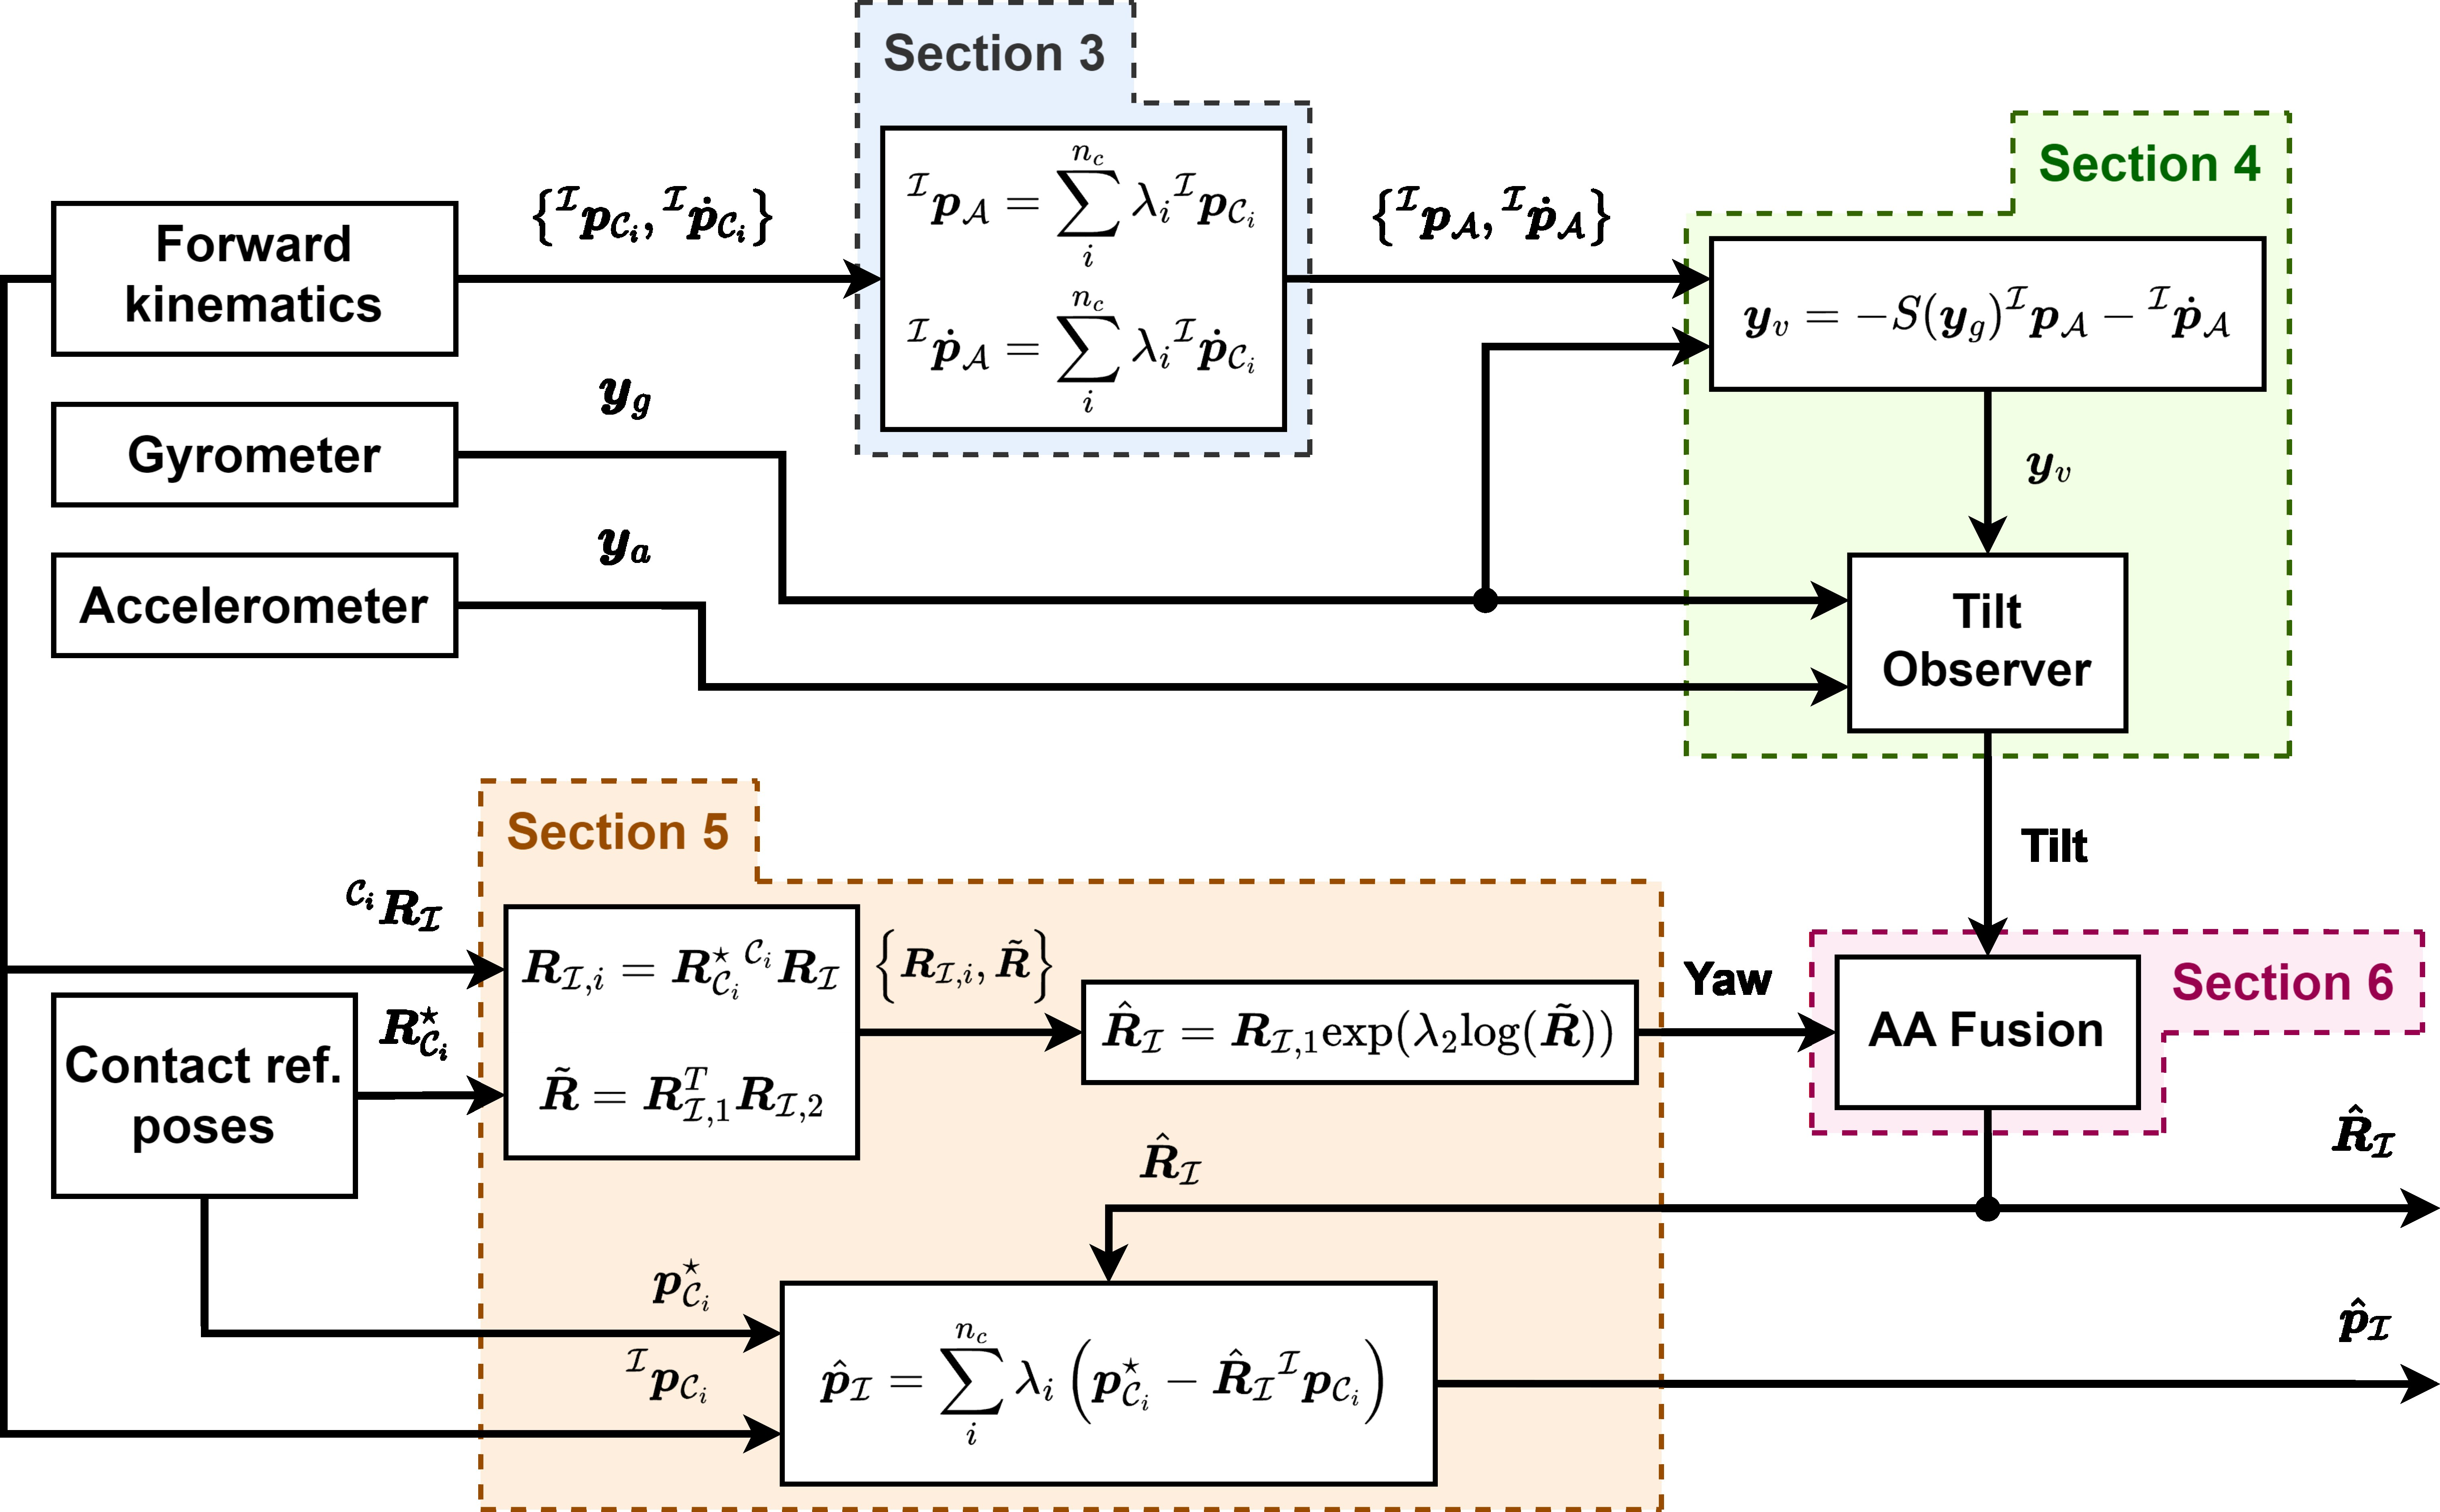
\includegraphics[width=0.65\textwidth]{summary.jpg}
        \label{fig:summary}
    }
      \hfill
    \subfloat[]{
        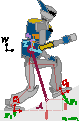
\includegraphics[width=0.20\textwidth]{framesAndAnchor.pdf}
        \label{fig:framesAndAnchor}
    }
    \caption{(a) Summary of {\scshape Valinor}'s pipeline. (b) Illustration of the anchor point position computation and of the reference frames used in {\scshape Valinor}. $\mathcal{W}$: world frame; $\mathcal{I}$: IMU frame; $\mathcal{C}_{i}$: frame of the $i$-th contact. For clarity, only the weighted average of the contact positions is shown. In this example, $\boldsymbol{F}_{2} = 2\boldsymbol{F}_{1}$ and so $\lambda_{2} = \frac{2}{3}$.}
\end{figure*}


\section{GENERAL NOTATIONS}
\begin{itemize}
    \item The general notation for kinematic variables is $^{1}\bigcirc_{2}$ , expressing the kinematics of the frame $2$ in the frame $1$. To simplify the notation, kinematics in the world frame are written without the $\mathcal{W}$ symbol: $^{\mathcal{W}}\bigcirc_{2}=\bigcirc_{2}$.
    \item We note $\hat{\boldsymbol{x}}$ the estimate of the variable $\boldsymbol{x}$.
    \item The world frame and the robot's IMU frame are denoted $\mathcal{W}$ and $\mathcal{I}$, respectively. The frame associated with the $i$-th contact is denoted $\mathcal{C}_{i}$. The anchor point, defined in Section~\ref{sec:anchor_point}, is denoted $\mathcal{A}$. 
    \item $\times$ is the cross-product operator. 
    \item We define $n_c$ the number of current contacts set with the environment.
    
\end{itemize} 



\section{DEFINITION OF THE ANCHOR POINT}\label{sec:anchor_point}
We define here the notion of anchor point, since it will be used extensively in the following sections. It is notably essential for the design of the Tilt Observer, as explained in Section~\ref{subsec:tiltMeas}.

The anchor point, denoted $\mathcal{A}$, is defined as a point attached to the robot and which is considered to have zero \emph{instantaneous} linear velocity in the world frame. This point does not need to be fixed in the robot frame as well, the only requirement is that its instantaneous position and linear velocity in the frame of the robot's floating base are known. 

Contacts with the environment provide naturally good sets of points known to the robot and having zero world velocity. With the no-slippage hypothesis, any point of a contact body would thus be suitable to define an anchor point. However, we need an anchor point that remains always defined and whose position is as continuous as possible, even when contacts are created and broken, as long as there is at least one contact established. Also, the no-slippage hypothesis can hold better for some points than others. For instance, when the contact forces are closer to Coulomb's friction cones the contact is more likely to slip.

To address these two requirements we determine the kinematics of that point through a weighted average of the kinematics of the current contacts, as shown in Figure~\ref{fig:framesAndAnchor}.  \\
The weighting coefficients are defined such that weaker contacts, which are prone to violate Coulomb's inequality and thus to slip, contribute less to the anchor point's kinematics computation. Given $mg_{0}$ the weight of the robot, we first compute for each contact $i$ the ratio $u_{i}$ of the normal force to the tangential force, measured by the force / torque sensor at the contact. The term $\epsilon$, arbitrarily small, allows to deal with the case where the tangential force is zero. The weighting coefficient $\lambda_{i}$ of the contact in the average is then computed:
\begin{equation}
    u_{i} = \frac{\boldsymbol{F}_{i,z}}{\sqrt{\boldsymbol{F}_{i,x}^2 + \boldsymbol{F}_{i,y}^2} + \epsilon mg_{0}}, \qquad \lambda_{i}=\frac{u_{i}}{\sum^{n_{c}}_{j=1}u_{i}}. \label{eq:ratio_ui}
\end{equation}
Based on this definition, we give the position and linear velocity of the anchor point in the IMU's frame:
\begin{align} 
&{^{\mathcal{I}}}\boldsymbol{p}_{\mathcal{A}} = \sum^{n_{c}}_{i} \lambda_{i}  {^{\mathcal{I}}} \boldsymbol{p}_{{\mathcal{C}}_{i}}, \label{eq:imuAnchorPos} \\
&{^{\mathcal{I}}} \dot{\boldsymbol{p}}_{\mathcal{A}} = \sum^{n_{c}}_{i} \lambda_{i}  {^{\mathcal{I}}} \dot{\boldsymbol{p}}_{{\mathcal{C}}_{i}}, \label{eq:imuAnchorVel}
\end{align} 
with ${^{\mathcal{I}}} \boldsymbol{p}_{{\mathcal{C}}_{i}}$ the position and ${^{\mathcal{I}}} \dot{\boldsymbol{p}}_{{\mathcal{C}}_{i}}$ the linear velocity of the $i$-th contact in the IMU's frame, which are directly provided by the robot's joint encoders and geometrical model. \\${^{\mathcal{I}}}\boldsymbol{p}_{\mathcal{A}}$ and ${^{\mathcal{I}}} \dot{\boldsymbol{p}}_{\mathcal{A}}$ are updated at each iteration. As explained in Section~\ref{subsec:tiltMeas}, by combining them with the zero-velocity assumption of the anchor point in the world frame and the gyrometer measurement, we obtain an algebraic estimate of the IMU velocity in the world frame.

It is important to note also that with this definition, although the anchor point is defined to have zero velocity in the world, its instantaneous position may still evolve over time.

% \begin{figure}[!t]
% \begin{center}
% 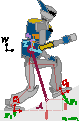
\includegraphics[width=0.4\columnwidth]{framesAndAnchor.pdf} 
% \vskip -0.5pc
% \caption{Illustration of the anchor point position computation and of the reference frames used in {\scshape Valinor}. $\mathcal{W}$: world frame; $\mathcal{I}$: IMU frame; $\mathcal{C}_{i}$: frame of the $i$-th contact. For clarity, only the weighted average of the contact positions is shown. In this example, $\boldsymbol{F}_{2} = 2\boldsymbol{F}_{1}$ and so $\lambda_{2} = \frac{2}{3}$.}\label{fig:framesAndAnchor}
% \end{center}
% \vskip -1.5pc
% \end{figure}


\section{Tilt Observer with proof of convergence}
\label{sec:tilt_observer}
The proposed estimator relies on a highly accurate estimate of the IMU's tilt provided by a complementary filter, introduced in~\cite{benallegue2020LyapunovStableOrientationEstimatorHumanoids}, which we will call \emph{Tilt Observer}. 

\subsection{Definition of the State Variables}
The Tilt Observer is able to provide estimates of the following two variables: 
\begin{itemize}
    \item $\boldsymbol{v}_{\mathcal{I}, l} \triangleq \boldsymbol{R}^{T}_{\mathcal{I}} \boldsymbol{v}_{\mathcal{I}} $ the linear velocity of the IMU's frame in the world frame, expressed in the frame of the IMU.
    \item $\boldsymbol{R}^{T}_{\mathcal{I}} \boldsymbol{e}_z$ the tilt of the IMU.
\end{itemize}
We thus define the state variables: 
\begin{alignat}{2}
&\boldsymbol{x}_{1} \triangleq \boldsymbol{v}_{\mathcal{I}, l} \quad &&, \boldsymbol{x}_{1} \in \mathbb{R}^{3}, \label{eq:x1} \\
&\boldsymbol{x}_{2} \triangleq \boldsymbol{R}^{T}_{\mathcal{I}} \boldsymbol{e}_z \quad &&, \boldsymbol{x}_{2} \in \mathbb{S}^{2}. \label{eq:x2}
\end{alignat} 
The set $\mathbb{S}^{2} \subset \mathbb{R}^{3}$ is the unit sphere centered at the origin, and defined as
\begin{equation}
    \mathbb{S}^{2} = \left\{ \boldsymbol{x} \in \mathbb{R}^{3} \vert \lVert \boldsymbol{x} \rVert=1 \right\}
\end{equation}


\subsection{Definition of the Measurements} \label{subsec:tiltMeas}
The measurements required by the Tilt Observer are:
\begin{itemize}
    \item $\boldsymbol{y}_{g}$ the signal of the IMU's gyrometer.
    \item $\boldsymbol{y}_{a}$ the signal of the IMU's accelerometer.
    \item $\boldsymbol{y}_{v}$ a measurement of $\boldsymbol{v}_{\mathcal{I}, l}$.
\end{itemize}
Since no sensor provides a direct measurement of $\boldsymbol{v}_{\mathcal{I}, l}$, we obtain $\boldsymbol{y}_{v}$ from an algebraic combination of gyrometer signal $\boldsymbol{y}_{a}$ and the position and velocity of the anchor point, ${^{\mathcal{I}}}\boldsymbol{p}_{\mathcal{A}}$  from~\eqref{eq:imuAnchorPos}
and ${^{\mathcal{I}}} \dot{\boldsymbol{p}}_{\mathcal{A}}$ from~\eqref{eq:imuAnchorVel} respectively, giving:
\begin{equation}
    \boldsymbol{y}_v = - \boldsymbol{y}_{g} \times {^{\mathcal{I}}}\boldsymbol{p}_{\mathcal{A}} - {^{\mathcal{I}}} \dot{\boldsymbol{p}}_{\mathcal{A}} \label{eq:yv}
\end{equation}

\subsection{Definition of the Filter} \label{subsec:tilt_def}
The state dynamics of our system can be written:
\begin{align} 
&\dot{\boldsymbol{x}}_{1} = - \boldsymbol{y}_{g} \times \boldsymbol{x}_{1} - g_{0}\boldsymbol{x}_{2} + \boldsymbol{y}_{a} , \label{eq:x1_dot} \\
&\dot{\boldsymbol{x}}_{2} = - \boldsymbol{y}_{g} \times  \boldsymbol{x}_{2}. \label{eq:x2_dot}
\end{align} 
with $g_{0}$ the gravitational acceleration constant. We write a complementary filter which uses the system's dynamics as a feed-forward, and corrects the estimated state using the velocity measurement $\boldsymbol{y}_{v}$:
\begin{empheq}[left= \empheqlbrace]{align}
    \dot{\hat{\boldsymbol{x}}}_{1} &= - \boldsymbol{y}_{g} \times \hat{\boldsymbol{x}}_{1} - g_{0} \hat{\boldsymbol{x}}_{2}^{\prime} + \boldsymbol{y}_{a} + \alpha_{1} (\boldsymbol{y}_{v} - \hat{\boldsymbol{x}}_{1}) \label{eq:tilt_dynamics_1} \\
    \dot{\hat{\boldsymbol{x}}}_{2}^{\prime} &= -  \boldsymbol{y}_{g} \times \hat{\boldsymbol{x}}_{2} - \frac{\alpha_{2}}{g_{0}} (\boldsymbol{y}_{v} - \hat{\boldsymbol{x}}_{1}) \label{eq:tilt_dynamics_2} \\
    \dot{\hat{\boldsymbol{x}}}_{2} &= - (\boldsymbol{y}_{g} - \gamma \hat{\boldsymbol{x}}_{2} \times \hat{\boldsymbol{x}}_{2}^{\prime})\times \hat{\boldsymbol{x}}_{2} \label{eq:tilt_dynamics_3}
\end{empheq}


$\hat{\boldsymbol{x}}_{1} $ is the estimate of $\boldsymbol{x}_{1} $. $\hat{\boldsymbol{x}}_{2}^{\prime}$ is an intermediate estimate of $\boldsymbol{x}_{2} $, which converges exponentially but is not restricted to lie on the sphere $\mathbb{S}^{2}$. This estimate drives the convergence of the final estimate $\hat{\boldsymbol{x}}_{2} $, which is explicitly projected onto $\mathbb{S}^{2}$ so as to respect its Lie group structure.
The positive scalar gains $\alpha_1$, $\alpha_2$ and $\gamma$ define the convergence rates of the three state estimates. Insights on their tuning are provided in~\cite{benallegue2023velocity}. Note that the filter's convergence guarantees hold regardless of the gains' tuning.

\subsection{Advantages of the Tilt Observer}
The use of a complementary filter for the Tilt Observer presents notable strengths in comparison to other methods like the commonly used Kalman Filter. First, it allows us to easily work in the frequency domain when determining the gains. This is particularly suitable for our model since the assumption of fixed contacts used to obtain the velocity measurement $\boldsymbol{y}_v$ is more valid in low frequency than in high frequency. In~\eqref{eq:tilt_dynamics_1}, we thus use the IMU measurements for the high frequency feed-forward of $\hat{\boldsymbol{x}}_{1}$, and $\boldsymbol{y}_v$ for its low frequency correction. Second, one iteration of the filter only consists in computing three equations, it also doesn't involve any matrix multiplication or inversion and is thus computationally extremely cheap, as will be shown in Section~\ref{subsec:computation_time}. Finally, the formulation as a complementary filter allows to conduct a convergence analysis of the estimation error, providing strong mathematical guarantees on the estimator's performances. Especially here, it has been shown in~\cite{benallegue2020LyapunovStableOrientationEstimatorHumanoids} that:
\begin{itemize}
    \item The dynamics of the estimation error is autonomous, and thus does not depend on the motion of the robot. 
    \item The intermediate estimator $\left\{\hat{\boldsymbol{x}}_{1}, \hat{\boldsymbol{x}}_{2}^{\prime} \right\}$ is \emph{globally exponentially stable}, with respect to the origin $\left(0,0\right)$.
    \item The full estimator is \emph{almost globally asymptotically stable}, and locally \emph{exponentially stable}. It provides a good filtering of noise and guarantees to respect the normality constraint.
\end{itemize}

\section{Leg Odometry for Position and Yaw Estimation} \label{sec:leg_odometry}

While the tilt of the IMU's frame in the world frame is estimated by the Tilt Observer, its position and yaw are obtained using Leg odometry. Once a contact $i$ is created, its \emph{reference} pose $\left\{ \boldsymbol{p}^{\star}_{\mathcal{C}_{i}}, \boldsymbol{R}^{\star}_{\mathcal{C}_{i}}\right\}$ in the world is obtained by forward kinematics from the estimated IMU's frame pose $\left\{ \hat{\boldsymbol{p}}_{\mathcal{I}}, \hat{\boldsymbol{R}}_{\mathcal{I}}\right\}$ :
\begin{align}
  \boldsymbol{R}^{\star}_{\mathcal{C}_{i}}  & = \hat{\boldsymbol{R}}_{\mathcal{I}}  {}^{\mathcal{I}} \boldsymbol{R}_{\mathcal{C}_{i}}  \text{ ,}\\
    \boldsymbol{p}^{\star}_{{\mathcal{C}}_{i}}   & = \hat{\boldsymbol{p}}_{\mathcal{I}} + \hat{\boldsymbol{R}}_{\mathcal{I}} {}^{\mathcal{I}}\boldsymbol{p}_{{\mathcal{C}}_{i}} ,
\end{align}
with $\left\{ {}^{\mathcal{I}}\boldsymbol{p}_{{\mathcal{C}}_{i}}, {}^{\mathcal{I}} \boldsymbol{R}_{\mathcal{C}_{i}} \right\}$ the pose of the $i$-th contact in the IMU's frame provided by the robot's geometrical model and joint encoders.
The contact's reference pose is then considered constant to enforce the contact's anchoring role, and used to recover the pose of the IMU's frame in the world frame. 
With the proposed pipeline, we thus leverage both the accuracy and mathematical guarantees provided by the Tilt Observer, and the robustness to drift provided by the Leg odometry. Similarly to the computation of the anchor point in Section~\ref{sec:anchor_point}, the contribution of contacts to the Leg odometry is weighted to trust more contacts which are the least prone to slippage, in order to mitigate its effect.

First, we estimate the IMU's orientation from contact information. For the two most reliable contacts\footnote{The two contacts with the highest ratio $u$ defined in~\eqref{eq:ratio_ui}.}, we compute the IMU frame's orientation from the contact's reference orientation. For each contact $i$, we write:
\begin{equation}
    \boldsymbol{R}_{\mathcal{I}, i} = \boldsymbol{R}^{\star}_{\mathcal{C}_{i}} {}^{\mathcal{C}_{i}} \boldsymbol{R}_{\mathcal{I}}, \label{eq:R_I_i}
\end{equation}
with ${}^{\mathcal{C}_{i}} \boldsymbol{R}_{\mathcal{I}}$ the orientation of the IMU's frame in the contact frame, provided by the robot's geometrical model and joint encoders.\\
We then compute the error between the obtained orientations, which is used to compute their weighted average, using the formalism defined by SO(3) the Lie group of rotation matrices:
\begin{align}
    &\tilde{\boldsymbol{R}} = \boldsymbol{R}^{T}_{\mathcal{I}, 1} \boldsymbol{R}_{\mathcal{I}, 2}  \\
 & \hat{\boldsymbol{R}}_{\mathcal{I}} = \boldsymbol{R}_{\mathcal{I}, 1} \text{exp} \left( \lambda_{2}\text{log} \left( \tilde{\boldsymbol{R}}\right)  \right). \label{eq:leg_odom_avg_ori}
\end{align}
exp and log are the \emph{exponential} and \emph{logarithm} maps of SO(3). We note that for small angles, we can use the approximation:
\begin{equation}
\text{log}\left(\tilde{\boldsymbol{R}}\right) \simeq \frac{1}{2} \left(\tilde{\boldsymbol{R}}-\tilde{\boldsymbol{R}}^{T}\right), \label{eq:log_small}
\end{equation}
Once the IMU's orientation $\hat{\boldsymbol{R}}_{\mathcal{I}}$ has been computed, we merge the corresponding yaw with the tilt estimated by the Tilt Observer using a new axis-agnostic fusion of tilt and yaw, that we describe in Section~\ref{sec:axisAgnostic}, which preserves the estimated tilt and its mathematical convergence guarantees with little computations.

The position of the IMU's frame in the world frame is then obtained from the $n_{c}$ contact reference poses: 
\begin{equation}
    \hat{\boldsymbol{p}}_{\mathcal{I}} = \sum^{n_{c}}_{i} \lambda_{i} \left( \boldsymbol{p}^{\star}_{{\mathcal{C}}_{i}} - \hat{\boldsymbol{R}}_{\mathcal{I}} {}^{\mathcal{I}}\boldsymbol{p}_{{\mathcal{C}}_{i}} \right). \label{eq:est_p_imu}
\end{equation}
We note that this position is obtained using the IMU's orientation estimate that merges the estimated tilt with the yaw coming from the odometry. It takes then full profit from the accurate tilt provided by the Tilt Observer.


%=====================================================================
\section{Tilt--Yaw Fusion}
\label{sec:axisAgnostic}
%=====================================================================

The Tilt Observer of Section~\ref{sec:tilt_observer} provides $\hat{\boldsymbol{x}}_{2}$,  an accurate
estimate of the IMU \emph{tilt} noted
\(
  \boldsymbol{\ell}=\boldsymbol{R}_{1}^{\top}\boldsymbol{e}_{z},
\)
while the contact–based Leg odometry of
Section~\ref{sec:leg_odometry} supplies an orientation \(\boldsymbol{R}_{2} = \hat{\boldsymbol{R}}_{\mathcal{I}}\), whose
yaw reflects the robot's heading.  We now merge these two pieces into a single rotation \(\boldsymbol{R}\), which would preserve our tilt estimate, especially its mathematical convergence guarantees.

%.....................................................................
\subsection{Why not Euler angles?}
%.....................................................................

Classically in these situations, we use the Euler angles representation of the rotations,
\(\boldsymbol{R}_{1}=R_{z}(\psi_{1})R_{y}(\theta_{1})R_{x}(\phi_{1})\) and
\(\boldsymbol{R}_{2}=R_{z}(\psi_{2})R_{y}(\theta_{2})R_{x}(\phi_{2})\),
the textbook fusion is
\begin{equation}
  \boldsymbol{R}_{\mathrm{cl}}
  =R_{z}(\psi_{2})\,R_{y}(\theta_{1})\,R_{x}(\phi_{1}).
  \label{eq:fusion_classic}
\end{equation}
This solution has two properties
\begin{itemize}
\item tilt is conserved, i.e. 
\(\boldsymbol{R}_{\mathrm{cl}}^{\top}\boldsymbol{e}_{z}=\boldsymbol{\ell}\).
\item among all rotations \(\hat{\boldsymbol{R}}\) such that
\(\hat{\boldsymbol{R}}^{\top}\boldsymbol{e}_{z}=\boldsymbol{\ell}\),
\(R_{\mathrm{cl}}\) minimises the horizontal error
\(
  \|
    \hat{\boldsymbol{R}}^{\top}\boldsymbol{e}_{x}-\boldsymbol{R}_{2}^{\top}\boldsymbol{e}_{x}
  \|^{2}.
\)
\end{itemize}


Despite its simplicity, \eqref{eq:fusion_classic} rests on two tacit
assumptions that are seldom met in the leg–inertial setting considered
here:

\begin{itemize}
\item The optimality of \eqref{eq:fusion_classic} is defined with
      respect to the IMU axis $\boldsymbol{e}_{x}$ only.  
      This makes sense when $\boldsymbol{e}_{x}$ \emph{is} the heading
      carrier, for example with a GPS-based heading for wheeled vehicles.  
      In practice the IMU can be installed with an arbitrary yaw
      offset, and our yaw information actually comes from leg odometry
      (average contact frames, Section~\ref{sec:leg_odometry}), not from
      that axis.  Treating $\boldsymbol{e}_{x}$ as ``special'' therefore
      introduces a systematic bias.

\item Because \eqref{eq:fusion_classic} uses a ZYX decomposition of
      $\boldsymbol{R}_{1}$, it inherits the Euler-angle singularity at
      $\theta_{1}= \pm 90^{\circ}$.  
      Exactly there the pitch axis aligns with
      $\boldsymbol{e}_{z}$, roll and yaw collapse, and the horizontal
      projection of $\boldsymbol{e}_{x}$ disappears, leaving the yaw
      numerically indeterminate.  
      Such attitudes are frequent in humanoids that perform
      multicontact motions.
\end{itemize}
To avoid these two issues we adopt an \emph{axis-agnostic} fusion that
uses solely the measured tilt $\boldsymbol{\ell}$, allows any horizontal
vector to encode yaw, and stays regular for all configurations except
the physically undefined case $\boldsymbol{\ell}=-\boldsymbol{e}_{z}$.
The construction is detailed next.

%---------------------------------------------------------------------
\subsection{Yaw without Euler angles}
\label{sec:yaw_no_euler}
%---------------------------------------------------------------------

The yaw contained in $\boldsymbol{R}_{2}$ can be extracted without decomposing the
matrix into Euler angles.  Let's denote the third column of $\boldsymbol{R}_{2}$ as $\boldsymbol{r}_{2}$.
This column describes the world coordinates of the body $\boldsymbol{z}$-axis, i.e $\boldsymbol{r}_{2}=\boldsymbol{R}_{2}\boldsymbol{e}_z$, which is not the tilt of $\boldsymbol{R}_{2}$. 
Using that row we build the horizontal vector
\begin{equation}
  \boldsymbol{m}_2
  =
  \begin{cases}
    \boldsymbol{e}_x, &
    \text{if } {r}_{2,x}^{2}+{r}_{2,y}^{2}\simeq0,\\[6pt]
      \dfrac{1}{\sqrt{{r}_{2,x}^{2}+{r}_{2,y}^{2}}} [{r}_{2,y}\;-{r}_{2,x}\;0]^{\top},
    & \text{otherwise.}
  \end{cases}
\end{equation}
where ${r}_{2,x}$ and ${r}_{2,y}$ are the first and second components of $\boldsymbol{r}_{2}$. 
The condition ${r}_{2,x}^{2}+{r}_{2,y}^{2}\simeq0$ occurs when the tilt $\boldsymbol{R}_{2}^T \boldsymbol{e}_z$ is vertical (upward or downward), so we take $\boldsymbol{m}=\boldsymbol{e_x}$ to avoid the singularity.
Otherwise, the vector $\boldsymbol{m}_2$ always exists and is unique.

Rotating $\boldsymbol{m}_2$ by $\boldsymbol{R}_{2}^T$
results in another vector
$\tilde{\boldsymbol{m}}_2=\boldsymbol{R}_{2}^T\boldsymbol{m}_2$, which is horizontal as well.
This means that  $\boldsymbol{m}_2$ is an invariant horizontal vector. 

We define the yaw of~$\boldsymbol{R}_{2}$, as the angle between these two vectors $\boldsymbol{m}_2$ and $\tilde{\boldsymbol{m}}_2$, which is computed as
\begin{equation}
  \theta
  =
  \operatorname{atan2}\Bigl(
     {m}_{2,x}\tilde{{m}}_{2,y}
    -{m}_{2,y}\tilde{{m}}_{2,x},\;
     {m}_{2,x}\tilde{{m}}_{2,x}
    +{m}_{2,y}\tilde{{m}}_{2,y}
  \Bigr),
  \label{eq:yaw_theta}
\end{equation}
where the $x$ and $y$ subscripts denote the first and second components of the corresponding vector. 
The use of horizontal invariant vectors to define the yaw angle guarantees that we only consider rotations around the vertical axis, giving the most sound definition of yaw.

When the tilt $\boldsymbol{R}_{2}^T \boldsymbol{e}_z$ is vertical, any horizontal vector is invariant. In such a case, taking $\boldsymbol{m}=\boldsymbol{e_x}$ amounts at mimicking Euler yaw angle. 
When this tilt is downward, meaning $\boldsymbol{R}_{2}$ is a rotation of $\pi$ around a horizontal axis, the concept of yaw itself is ill-defined. When the tilt is upward, any horizontal vector gives the same yaw, so using Euler's yaw angle by taking  $\boldsymbol{m}_2=\boldsymbol{e_x}$ is a valid choice.

 Fortunately we don't have to compute this angle explicitly to perform the merge. It can be done directly using the tilt $\boldsymbol{\ell}$ and the second matrix $\boldsymbol{R}_{2}$.

%---------------------------------------------------------------------
\subsection{Axis-agnostic triad fusion}
\label{sec:triad_fusion}
%---------------------------------------------------------------------

\subsubsection{Select a proper reference vector}
Similarly to the yaw computation above, we start with the selection of the reference vector. However, the fusion makes this step slightly more subtile than just identifying the yaw of a single matrix. This is because the two rotations could have a very different tilt. This could lead the tilt vector $\boldsymbol{\ell}$ to be nearly colinear with the rotated horizontal invariant vector $\boldsymbol{R}_{2}^T\boldsymbol{m}_2$. This would make the fusion singular. 

The solution is to find a reference vector that is both horizontal and orthogonal to the real up direction $\boldsymbol{r}=\boldsymbol{R}_{2}\boldsymbol{\ell}=[v_{x}\;v_{y}\;v_{z}]^{\top}$.
Consequently, a proper reference vector can be defined as
\[
  \boldsymbol{m}
  =
  \begin{cases}
    \boldsymbol{m}_2, &
      \text{if } v_{x}^{2}+v_{y}^{2}\simeq0,\\[6pt]
    \dfrac{1}{\sqrt{v_{x}^{2}+v_{y}^{2}}}\,[v_{y}\;-v_{x}\;0]^{\top},
    & \text{otherwise.}
  \end{cases}
\]
The degenerate case occurs only when $\boldsymbol{r}$ is vertical, corresponding to $\boldsymbol{R}_{2}^{T}\boldsymbol{e}_{z} = \boldsymbol{\ell}$, which means the rotations nearly have the same tilt. In this situation we know that $\boldsymbol{\ell}$ and $\boldsymbol{R}_{2}^T\boldsymbol{m}_2$ are nearly orthogonal. We thus safely use the yaw angle definition of the previous section.  

We define the vector $\boldsymbol{m}$ expressed in the frame of $\boldsymbol{R}_{2}$ as 
$\boldsymbol{m}_{l}=R_{2}^{\top}\boldsymbol{m}$.


\subsubsection{ Build two right-handed bases.}
Using cross products, form
\[
  \boldsymbol{B}_{1}
  =
  \left[
    \boldsymbol{m}\times\boldsymbol{e}_{z}\quad
    \boldsymbol{e}_{z}\times\boldsymbol{m}\times\boldsymbol{e}_{z}\quad
    \boldsymbol{e}_{z}
  \right],
\]
\[
  \boldsymbol{B}_{2}
  =
  \left[
    \frac{\boldsymbol{m}_{l}\times\boldsymbol{\ell}}
         {\|\boldsymbol{m}_{l}\times\boldsymbol{\ell}\|}\quad
    \frac{\boldsymbol{\ell}\times\boldsymbol{m}_{l}\times\boldsymbol{\ell}}
         {\|\boldsymbol{m}_{l}\times\boldsymbol{\ell}\|}\quad
    \boldsymbol{\ell}
  \right].
\]
Each matrix is orthonormal: the first column is the chosen horizontal
vector, the third column is the vertical direction, and the second
column completes a right-handed frame.

\subsubsection{ Fuse tilt and yaw.}
The desired rotation is obtained by rotating from the basis
$\{\boldsymbol{m}_{2},\cdot,\boldsymbol{\ell}\}$ to
$\{\boldsymbol{m},\cdot,\boldsymbol{e}_{z}\}$:
\begin{equation}
  \boldsymbol{R} = \boldsymbol{B}_{1}\,\boldsymbol{B}_{2}^{\top}.
  \label{eq:fused_R}
\end{equation}



%.....................................................................
\subsection{Properties}
%.....................................................................

The rotation obtained with \eqref{eq:fused_R} shows the following
properties:

\begin{itemize}
  \item \emph{Tilt preservation}:  
        \(\boldsymbol{R}^{\top}\boldsymbol{e}_{z}=\boldsymbol{\ell}\).

  \item \emph{Optimal horizontal alignment}:  
        for any rotation \(\hat{\boldsymbol{R}}\) satisfying
        \(\hat{\boldsymbol{R}}^{\top}\boldsymbol{e}_{z}=\boldsymbol{\ell}\),
        the choice \eqref{eq:fused_R} minimises
        \[
          \bigl\|
             \hat{\boldsymbol{R}}^{\top}\boldsymbol{m}-\boldsymbol{m}_{l}
          \bigr\|^{2}.
        \]
        The proof follows exactly the one–parameter maximisation used
        for the Euler fusion, but with the task-specific direction
        \(\boldsymbol{m}\) in place of the body axis
        \(\boldsymbol{e}_{x}\).

  \item \emph{Singularity}:  
        the construction is undefined only when
        \(\boldsymbol{\ell}=-\boldsymbol{e}_{z}\); at that upside-down
        pose yaw itself has no meaning.

  \item \emph{Computation}:  
        implementation requires only vector cross products and
        normalisations, with no Euler-angle extraction, keeping the cost
        compatible with real-time embedded execution.
\end{itemize}

The axis-agnostic fusion is therefore adopted as the default in {\scshape Valinor}; it avoids the arbitrary preference for the body axis \(\boldsymbol{e}_{x}\), takes into account the difference of tilt and avoids the gimbal-lock issues of \eqref{eq:fusion_classic}. 





\section{Experimental Evaluation}~\label{sec:exps}

We identified the following criteria that a state estimator should satisfy to serve in our intended use case, namely, providing feedback for remote control \cite{Grandia2024DesignControlBipedalRoboticCharacter} or task planning and execution in the robot's local workspace \cite{Tsuru2023OnlineMulticontactReplanningHumanoid}:
\begin{itemize}[label={}, leftmargin=1em]
  \item \textbf{Criterion}\,\critnum{1}\, High computation speed, to leave more processing time for the rest of the pipeline.
  \item \textbf{Criterion}\,\critnum{2}\, Accurate tilt and local lateral (horizontal) velocity estimation, which are crucial for stabilization.
  \item \textbf{Criterion}\,\critnum{3}\, Low local drift (over small displacements) in translation and yaw. This would correlate with lower asbolute drift, but the latter cannot be used as a metric because of its lower determinism by proprioceptive odometry.
\end{itemize}

\noindent The experiments presented in this Section assess {\scshape Valinor} based on these criteria. We compare it with the Right-Invariant EKF (RI-EKF) from~\cite{Hartley2020RIEKF}, a state-of-the-art method for legged robot proprioceptive odometry. This estimator has demonstrated its effectiveness in practical applications, notably as real-time feedback for remote control~\cite{Grandia2024DesignControlBipedalRoboticCharacter}. It is therefore particularly relevant to compare ourselves to this method.

\subsection{Description of the experiments}

{\scshape Valinor} and the RI-EKF have been evaluated across two experimental scenarios on two different humanoid robots\footnote{We used the dataset built to evaluate the Kinetics Observer in~\cite{Demont2024KineticsObserver}}:
\begin{itemize}
    \item Experiment 1: A walk on a flat ground over about 18 meters with the robot RHP Friends~\cite{Benallegue2025RhpFriendsJRL}, as shown in Figure~\ref{fig:traj_friends}. This experiment was repeated 5 times, for a total distance of about 90 meters.
    \item Experiment 2: A multi-contact motion over about 2 meters with the robot HRP-5P~\cite{Kaneko2019Hrp5}. This motion involved an additional contact at the robot's left hand, and non-coplanar contacts on tilted obstacles, as shown in Figures~\ref{fig:traj_hrp5} and~\ref{fig:hrp5_motion}. This experiment was repeated 4 times for a total distance of about 8 meters.
\end{itemize}




\begin{figure}[!ht]
    \centering
    \subfloat[]{
        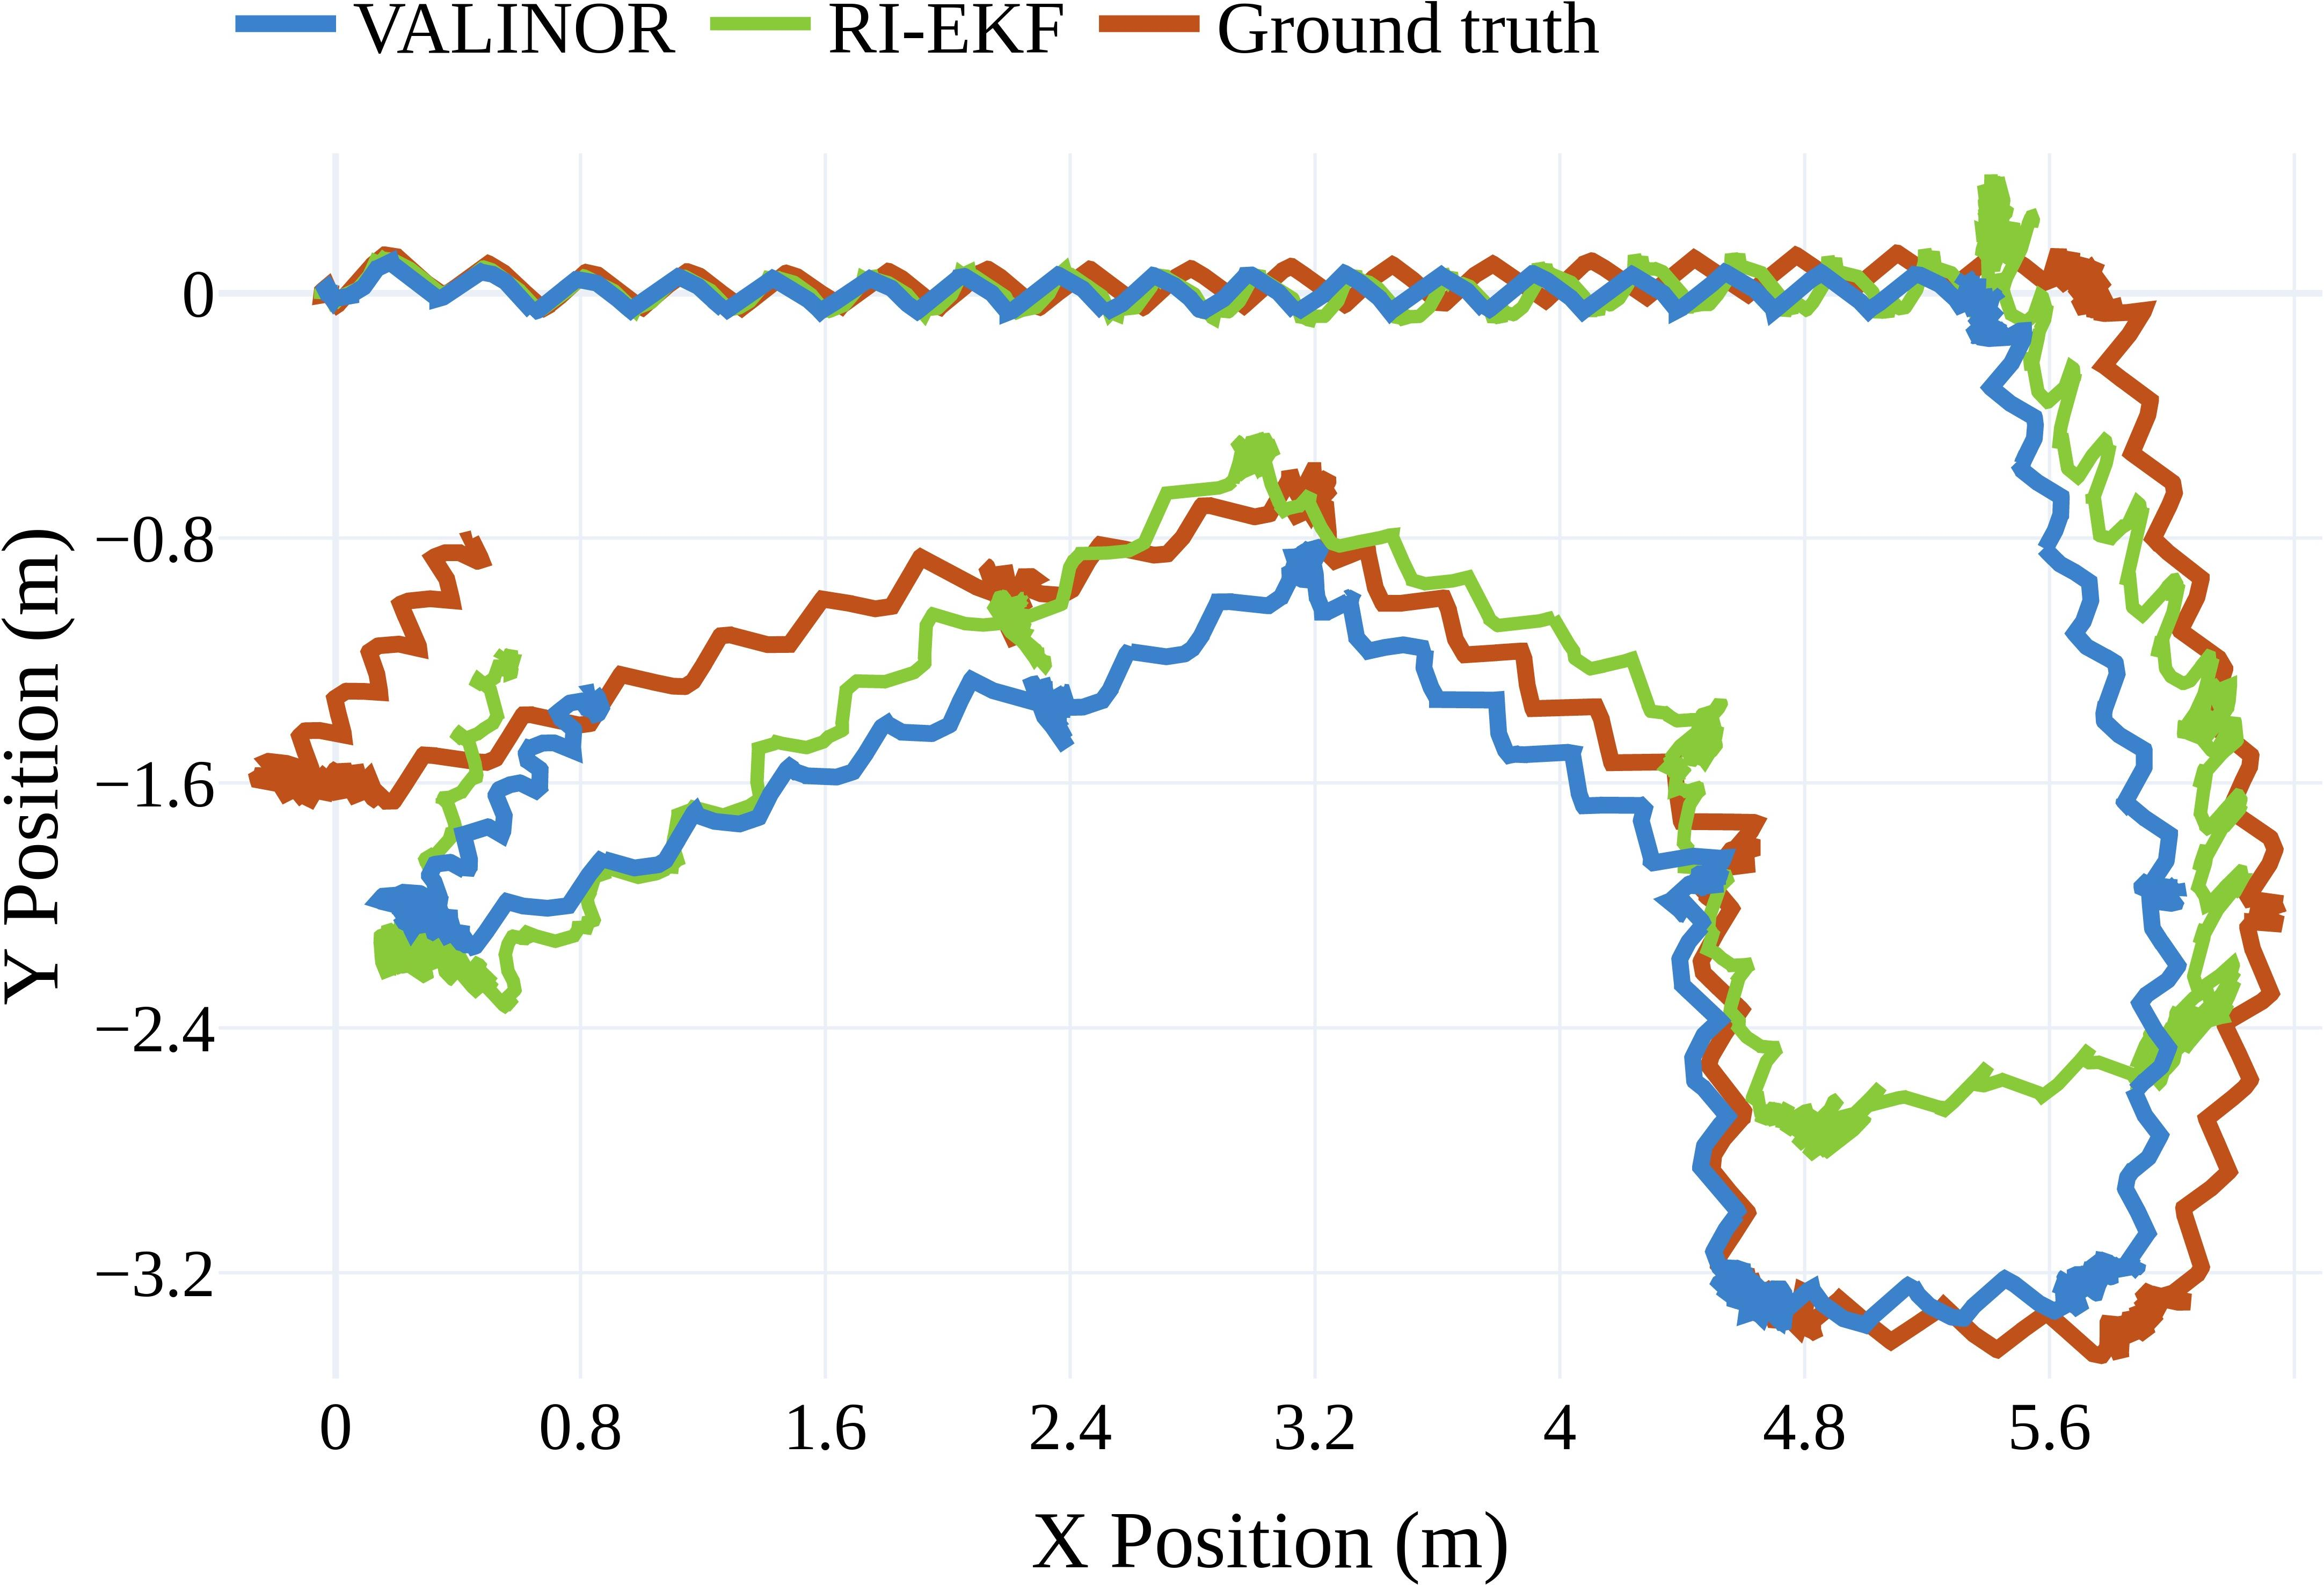
\includegraphics[width=0.85\columnwidth]{trajectory_rhps1.jpg}
        \label{fig:traj_friends}
    }\\[-1ex]
    \subfloat[]{
        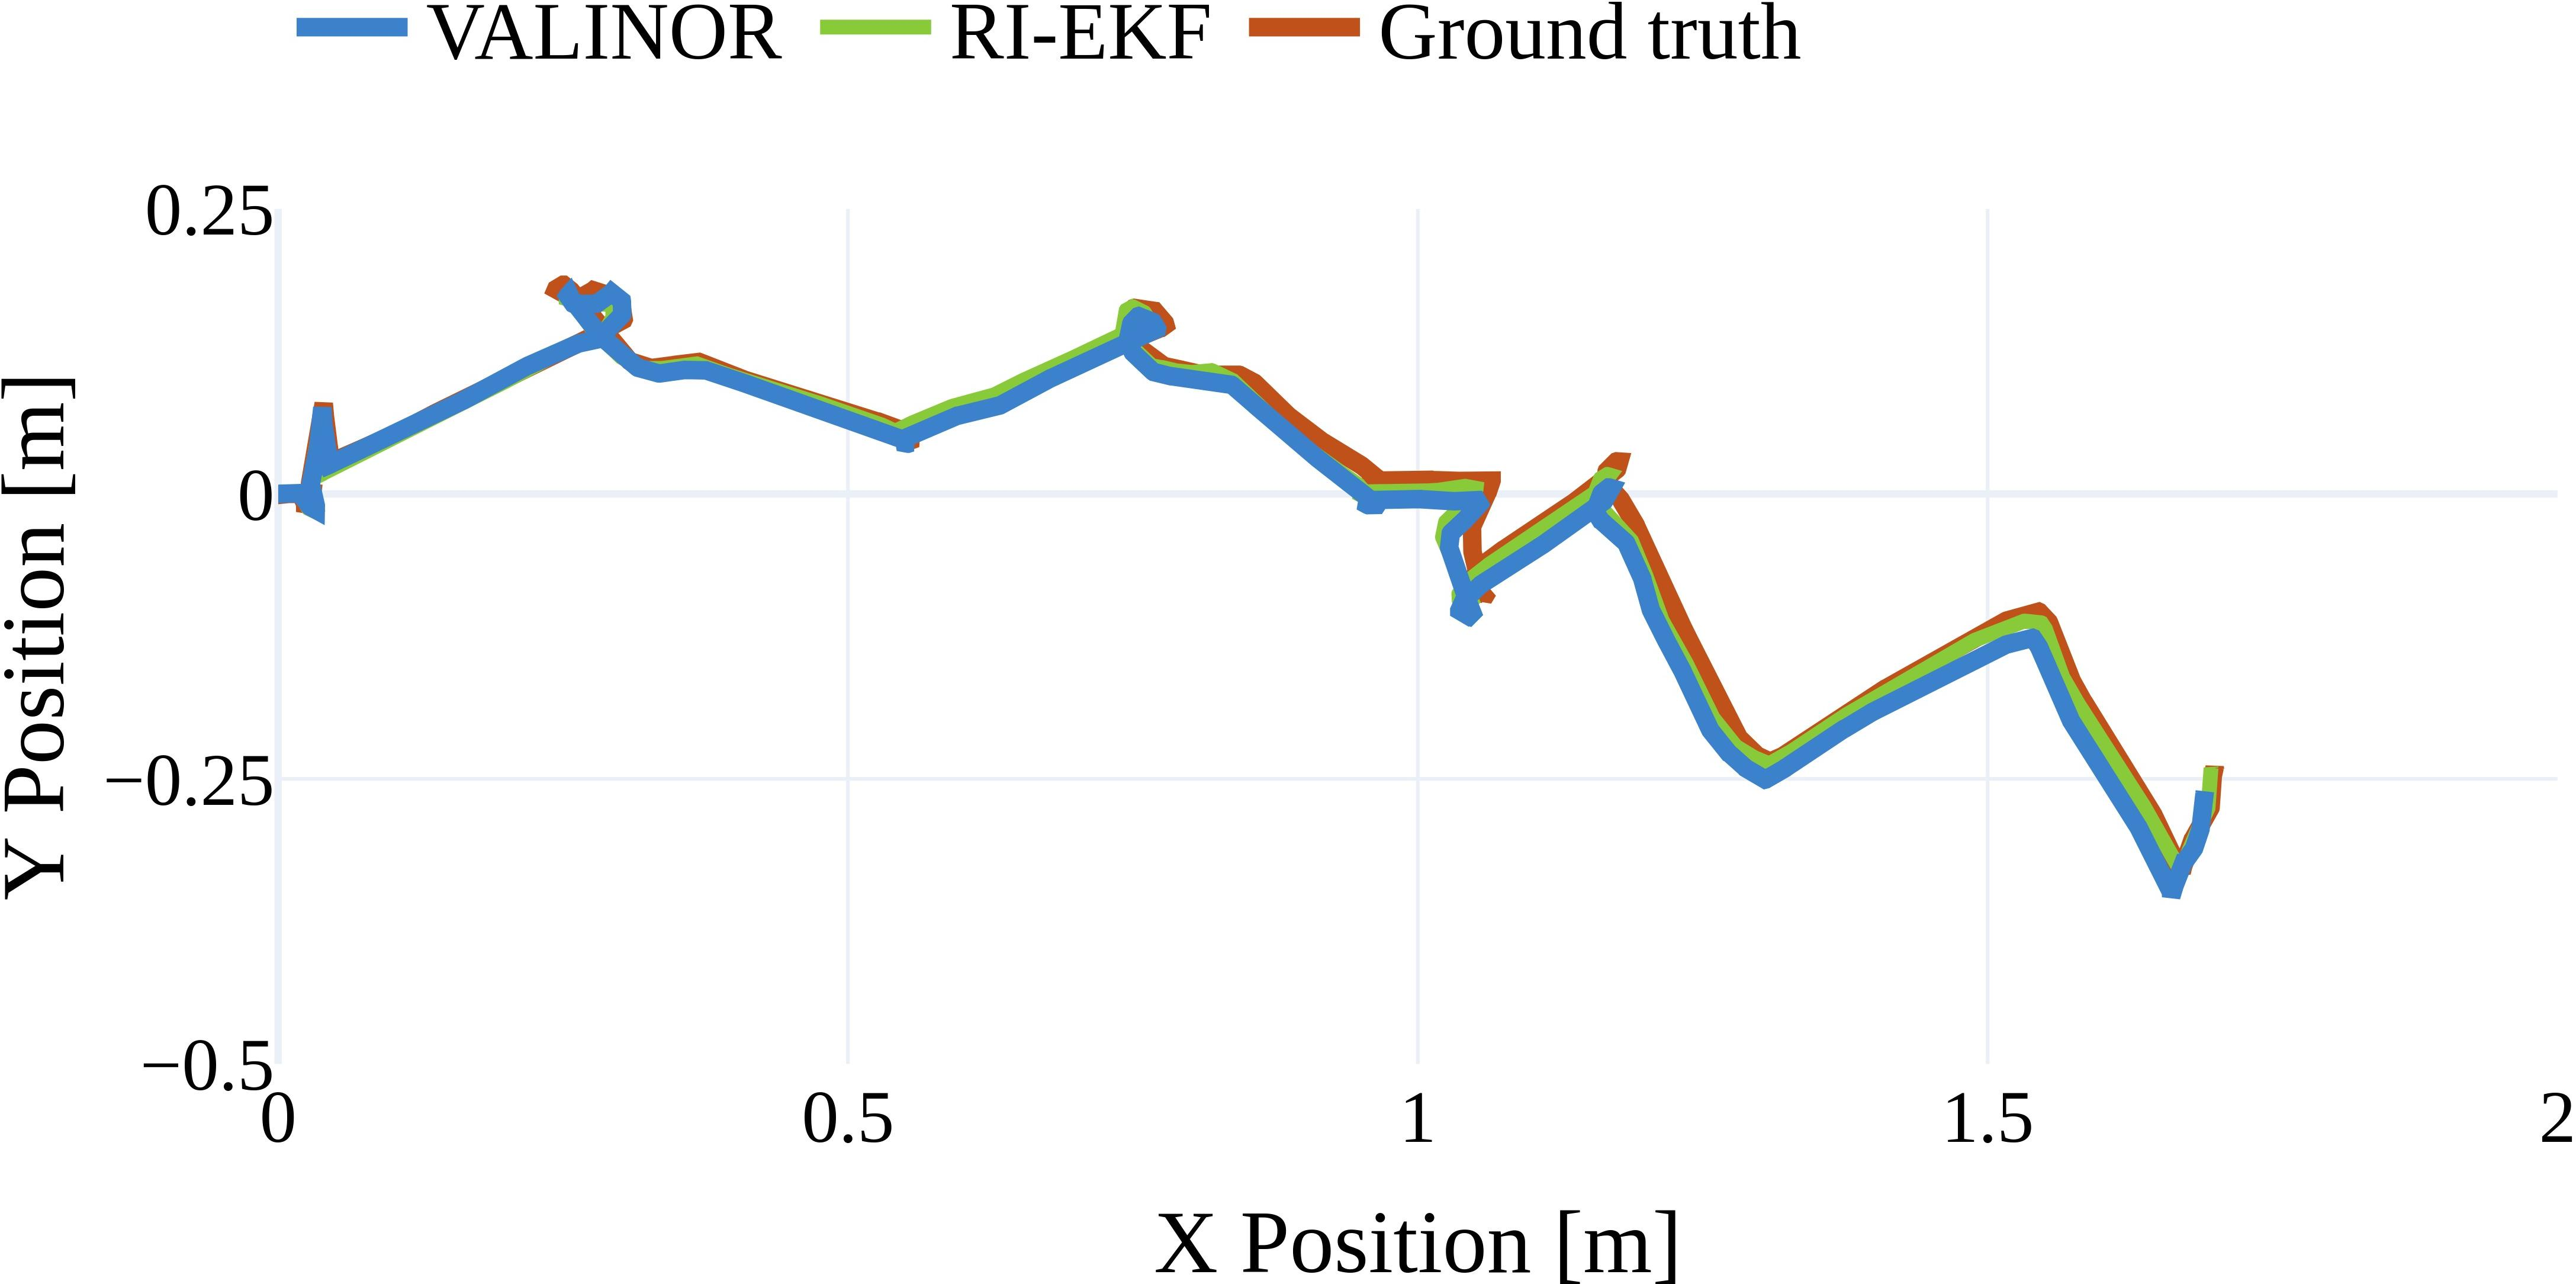
\includegraphics[width=0.85\columnwidth]{trajectory_hrp5.jpg}
        \label{fig:traj_hrp5}
    }\\[-1ex]
    \subfloat[]{
        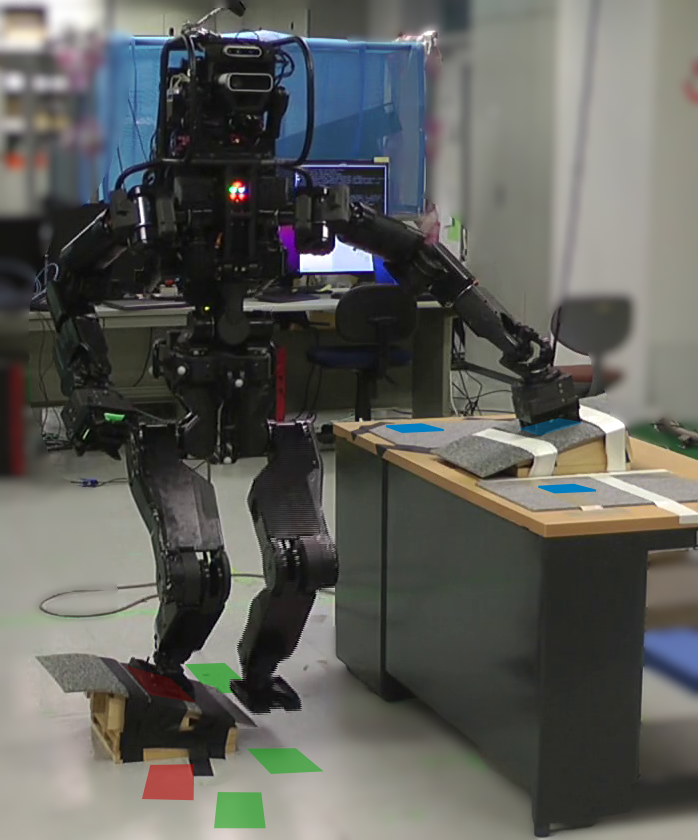
\includegraphics[width=0.45\columnwidth]{multiContactExpe.jpg}
        \label{fig:hrp5_motion}
    }
    \caption{Top views of the ground truth / estimated trajectories of the robot's pelvis during: (a) the first walk on flat ground (b) the multi-contact motion. The robot starts at the point (0,0) and walks towards the $\boldsymbol{x}$ direction. (c) HRP-5P performing the multi-contact motion. Contact imprints are represented by colored trapezoids. In red: Right foot. In green: Left foot. In blue: Left hand.  }
    \label{fig:flat-odom-rphs1}
\end{figure}


\subsection{Experimental Results}

\subsubsection{Computational Performance Evaluation}\label{subsec:computation_time}

To evaluate the computation speed performance of {\scshape Valinor}, we compared its average computation time per iteration over the four multi-contact experiments (involving three contacts), to that of the RI-EKF. Both estimators were run on the same laptop, equipped with an Intel Xeon E-2176M CPU (2.70GHz x 12). In average, an iteration of {\scshape Valinor} was computed in 2.547 \textmu s, against 19.315 \textmu s for the RI-EKF. The proposed method is thus more than 7.5 times faster than the state-of-the-art estimator. Across all sequences, the average computation times had a standard deviation of 0.043 \textmu s, indicating consistency from one sequence to another. We note that an additional contact in {\scshape Valinor} implies only minor additional computations in Eqs.~\eqref{eq:ratio_ui}, \eqref{eq:imuAnchorPos},\eqref{eq:imuAnchorVel}, and \eqref{eq:est_p_imu}, making our method highly scalable with respect to the number of contacts.


\subsubsection{Estimation Accuracy Evaluation} ~\label{subsec:est_accur_eval}


In both experiments, the odometry performance of {\scshape Valinor} and of the RI-EKF are evaluated using the ground truth trajectory of the robot's pelvis (to which the IMU is fixed on both robots), provided by a motion capture system (OptiTrack, 16 Prime\textsuperscript{X} with 13 cameras). The pose of the IMU's frame, estimated by both estimators, is transformed into that of the pelvis using simple rigid body transformation. For fairness in the comparison, both estimators receive the same contact state information, from a Schmitt Trigger on the Ground Reaction Force (with thresholds set to 10\% and 15\% of the robot's weight).
Since the focus is on accuracy in local translations and yaw (Criterion \critnum{3}), performance is assessed using the Relative Error (RE), as defined in~\cite{Zhang2018QuantitativeTrajectoryEvaluation}. The latter evaluates the estimation drift over segments of fixed distances. It is particularly relevant here, as it provides valuable and easily interpretable insight into the estimator's expected local accuracy without being affected by global drift. The error $e_{\boldsymbol{\ell}}$ on the tilt estimate is computed using $e_{\boldsymbol{\ell}} = \text{arccos}\left(\boldsymbol{\ell}_{gt}^{T} \hat{\boldsymbol{\ell}} \right)$, with $\boldsymbol{\ell}_{gt}$ the ground truth tilt, and $\hat{\boldsymbol{\ell}}$ the estimated one. 

Finally, local linear velocity estimation is assessed using the Mean Absolute Error between the estimated velocity and the ground truth, the latter obtained by finite differences from the ground-truth position, filtered with a zero-phase low-pass filter.

Table~\ref{tab:estimation_eval} regroups the evaluation results during the two experiments on real robots. The presented errors are computed over all sequences in each scenario: 5 for the walk on flat ground, and 4 for the multi-contact motion.


% We compute the Relative Error for lateral ($\boldsymbol{x}, \boldsymbol{y}$) and vertical ($\boldsymbol{z}$) translations separately, since these components are generally influenced by different factors. Accuracy in lateral translation would mainly rely on that of local displacements and of local yaw estimation, whereas accuracy in vertical translations would be affected by the accuracy of the vertical local displacement estimation, of the tilt, and the reliability of the contact height initialization. Similarily, angular errors in tilt and yaw are also evaluated independently.




\begin{table*}[h!] 
\vskip -0.75pc
\setlength{\extrarowheight}{1ex}
\addtolength{\tabcolsep}{-0.4em}
\caption{Mean and standard deviation (in parentheses) of the error on the estimations by {\scshape Valinor} and the RI-EKF, during the two experiments on real robots. The 1 m and the 0.3 m Relative Errors are presented for the walk on flat ground and the multi-contact motion, respectively. The best result for each metric is highlighted in bold.} \label{tab:estimation_eval}
\begin{center}
\vskip -1.25pc
{\footnotesize
    \begin{center}
        \begin{tabu}to\linewidth{| X[c] | X[c] | X[c] | X[c] | X[c] | X[c] | X[c] | X[c] |}
            \hline
            \multicolumn{2}{|c|}{}       &       \multicolumn{2}{c|}{RE Translation [m]}         &    \multicolumn{2}{c|}{RE Orientation [\textdegree] }  &    \multicolumn{2}{c|}{Linear velocity [$\text{m.s}^{-1}$]}     \\     
            \cline{3-8}
            \multicolumn{2}{|c|}{}  &     Lateral \{$\boldsymbol{x}, \boldsymbol{y}$\}   &      Vertical    $\boldsymbol{z}$      &    Tilt      &     Yaw    &  Lateral  \{$\boldsymbol{x}, \boldsymbol{y}$\}  &  Vertical  $\boldsymbol{z}$\\ 
            
            \tabucline[1.3pt]{-}
            
            Walk on  & {\scshape Valinor}   &    \textbf{\getErrorResult{Flatodometry}{Tilt}{Relerror}{Transxy}{Meanabs}} (\getErrorResult{Flatodometry}{Tilt}{Relerror}{Transxy}{Std}) &   \getErrorResult{Flatodometry}{Tilt}{Relerror}{Transz}{Meanabs}  (\getErrorResult{Flatodometry}{Tilt}{Relerror}{Transz}{Std})   &     \textbf{\getErrorResult{Flatodometry}{Tilt}{Relerror}{Tilt}{Meanabs}}  (\getErrorResult{Flatodometry}{Tilt}{Relerror}{Tilt}{Std})    &     \getErrorResult{Flatodometry}{Tilt}{Relerror}{Yaw}{Meanabs}  (\getErrorResult{Flatodometry}{Tilt}{Relerror}{Yaw}{Std})    &  \getErrorResult{Flatodometry}{Tilt}{Velerror}{EstimateXy}{Meanabs}   (\getErrorResult{Flatodometry}{Tilt}{Velerror}{EstimateXy}{Std})   &   \textbf{\getErrorResult{Flatodometry}{Tilt}{Velerror}{EstimateZ}{Meanabs}}  (\getErrorResult{Flatodometry}{Tilt}{Velerror}{EstimateZ}{Std}) \\ 
            \cline{2-8}
            flat ground &  RI-EKF~\cite{Hartley2020RIEKF} & \getErrorResult{Flatodometry}{Hartley}{Relerror}{Transxy}{Meanabs} (\getErrorResult{Flatodometry}{Hartley}{Relerror}{Transxy}{Std}) & \textbf{\getErrorResult{Flatodometry}{Hartley}{Relerror}{Transz}{Meanabs}} (\getErrorResult{Flatodometry}{Hartley}{Relerror}{Transz}{Std})     &  \getErrorResult{Flatodometry}{Hartley}{Relerror}{Tilt}{Meanabs}  (\getErrorResult{Flatodometry}{Hartley}{Relerror}{Tilt}{Std})    &    \textbf{\getErrorResult{Flatodometry}{Hartley}{Relerror}{Yaw}{Meanabs}}  (\getErrorResult{Flatodometry}{Hartley}{Relerror}{Yaw}{Std})  &  \textbf{\getErrorResult{Flatodometry}{Hartley}{Velerror}{EstimateXy}{Meanabs}}   (\getErrorResult{Flatodometry}{Hartley}{Velerror}{EstimateXy}{Std})  &   \getErrorResult{Flatodometry}{Hartley}{Velerror}{EstimateZ}{Meanabs}  (\getErrorResult{Flatodometry}{Hartley}{Velerror}{EstimateZ}{Std}) \\

            \tabucline[1.3pt]{-}
            Multi-contact &   {\scshape Valinor}  &  \textbf{\getErrorResult{Multicontact}{Tilt}{Relerror}{Transxy}{Meanabs}} (\getErrorResult{Multicontact}{Tilt}{Relerror}{Transxy}{Std})  &  \textbf{\getErrorResult{Multicontact}{Tilt}{Relerror}{Transz}{Meanabs}}  (\getErrorResult{Multicontact}{Tilt}{Relerror}{Transz}{Std})  &    \textbf{\getErrorResult{Multicontact}{Tilt}{Relerror}{Tilt}{Meanabs}}  (\getErrorResult{Multicontact}{Tilt}{Relerror}{Tilt}{Std})   &    \textbf{\getErrorResult{Multicontact}{Tilt}{Relerror}{Yaw}{Meanabs}}  (\getErrorResult{Multicontact}{Tilt}{Relerror}{Yaw}{Std})    &  \getErrorResult{Multicontact}{Tilt}{Velerror}{EstimateXy}{Meanabs}  (\getErrorResult{Multicontact}{Tilt}{Velerror}{EstimateXy}{Std})   &   \textbf{\getErrorResult{Multicontact}{Tilt}{Velerror}{EstimateZ}{Meanabs}}  (\getErrorResult{Multicontact}{Tilt}{Velerror}{EstimateZ}{Std}) \\ 
            \cline{2-8}     
            motion   & RI-EKF~\cite{Hartley2020RIEKF}  &  \getErrorResult{Multicontact}{Hartley}{Relerror}{Transxy}{Meanabs} (\getErrorResult{Multicontact}{Hartley}{Relerror}{Transxy}{Std})  &   \getErrorResult{Multicontact}{Hartley}{Relerror}{Transz}{Meanabs}  (\getErrorResult{Multicontact}{Hartley}{Relerror}{Transz}{Std})   &    \getErrorResult{Multicontact}{Hartley}{Relerror}{Tilt}{Meanabs}   (\getErrorResult{Multicontact}{Hartley}{Relerror}{Tilt}{Std})  &    \getErrorResult{Multicontact}{Hartley}{Relerror}{Yaw}{Meanabs}  (\getErrorResult{Multicontact}{Hartley}{Relerror}{Yaw}{Std})  &  \textbf{\getErrorResult{Multicontact}{Hartley}{Velerror}{EstimateXy}{Meanabs}}  (\getErrorResult{Multicontact}{Hartley}{Velerror}{EstimateXy}{Std})   &   \getErrorResult{Multicontact}{Hartley}{Velerror}{EstimateZ}{Meanabs} (\getErrorResult{Multicontact}{Hartley}{Velerror}{EstimateZ}{Std}) \\
            \hline     
        \end{tabu}
    \end{center}
}
\end{center}
\vskip -0.25pc
\end{table*}


Based on the obtained results, we observe that the relative strengths of both estimators were consistent across the two experiments. In the following, we detail these strengths, indicating the number of the criterion to which each is favorable in a circle.
\begin{itemize}
    \item {\scshape Valinor} estimated local lateral translations {\footnotesize\critnum{3}} more accurately than the RI-EKF in both experiments, improving the estimation by over 30\% and 40\%, respectively. Additionally, as visible in Figure~\ref{fig:pose_rhps1}, it improved the estimation of the tilt {\footnotesize\critnum{2}} by about 28\% in Experiment 1 and by 60\% in Experiment 2, reaching an average error of only 0.23\textdegree. For both translations and tilt estimates, our method displayed a significantly lower standard deviation of the error, proving an improved estimation consistency. 
    \item The RI-EKF estimated local lateral velocities {\footnotesize\critnum{2}} and yaw {\footnotesize\critnum{3}} more accurately than {\scshape Valinor} during Experiment 1, with 20\% and 16\% smaller errors, but both estimators displayed comparable performance in both estimates during Experiment 2.
    \item Both estimators showed similar performance in vertical translation {\footnotesize\critnum{3}} and velocity estimation. 
\end{itemize}
To elaborate on the vertical translation results, one can notice in Figure~\ref{fig:pose_rhps1} that both estimators drifted during the walk on flat ground, which involved a large number of steps. One contributing factor is the quality of the pitch estimation, an error in pitch estimation causing drift during forward walking. Another factor, inherent to Leg odometry, is its reliance on the quality of the contact detection. For example, systematically detecting contacts too early or too late can cause drift on each step, notably due to the robot's structural deformation under contact forces. In general use, this vertical drift could be reduced by tuning the contact detection threshold, which is arbitrarily set. However, to ensure a fair comparison, we kept the threshold unchanged and left this point for discussion. Moreover, absolute drift is not a reliable metrics for proprioceptive odometry (see Criterion \critnum{3}).

To conclude, both {\scshape Valinor} and the RI-EKF displayed relative strengths with respect to heach other, with regard to the criteria we defined. Overall, they provided highly satisfactory estimation performance which makes them well suited for local task planning and execution. Without the use of any exteroceptive sensors, their errors in translation estimates remain of the order of the centimeter per meter walked, those in orientation estimates remain around 1\textdegree \ per meter walked, and finally those in velocity estimates remain below 2 cm.s$^{-1}$. \\
It is noteworthy that, while reducing the computation time by more than a factor 7.5, {\scshape Valinor} could consistently improve tilt and lateral translation estimation significantly.

\begin{figure*}[!ht]
\begin{center}
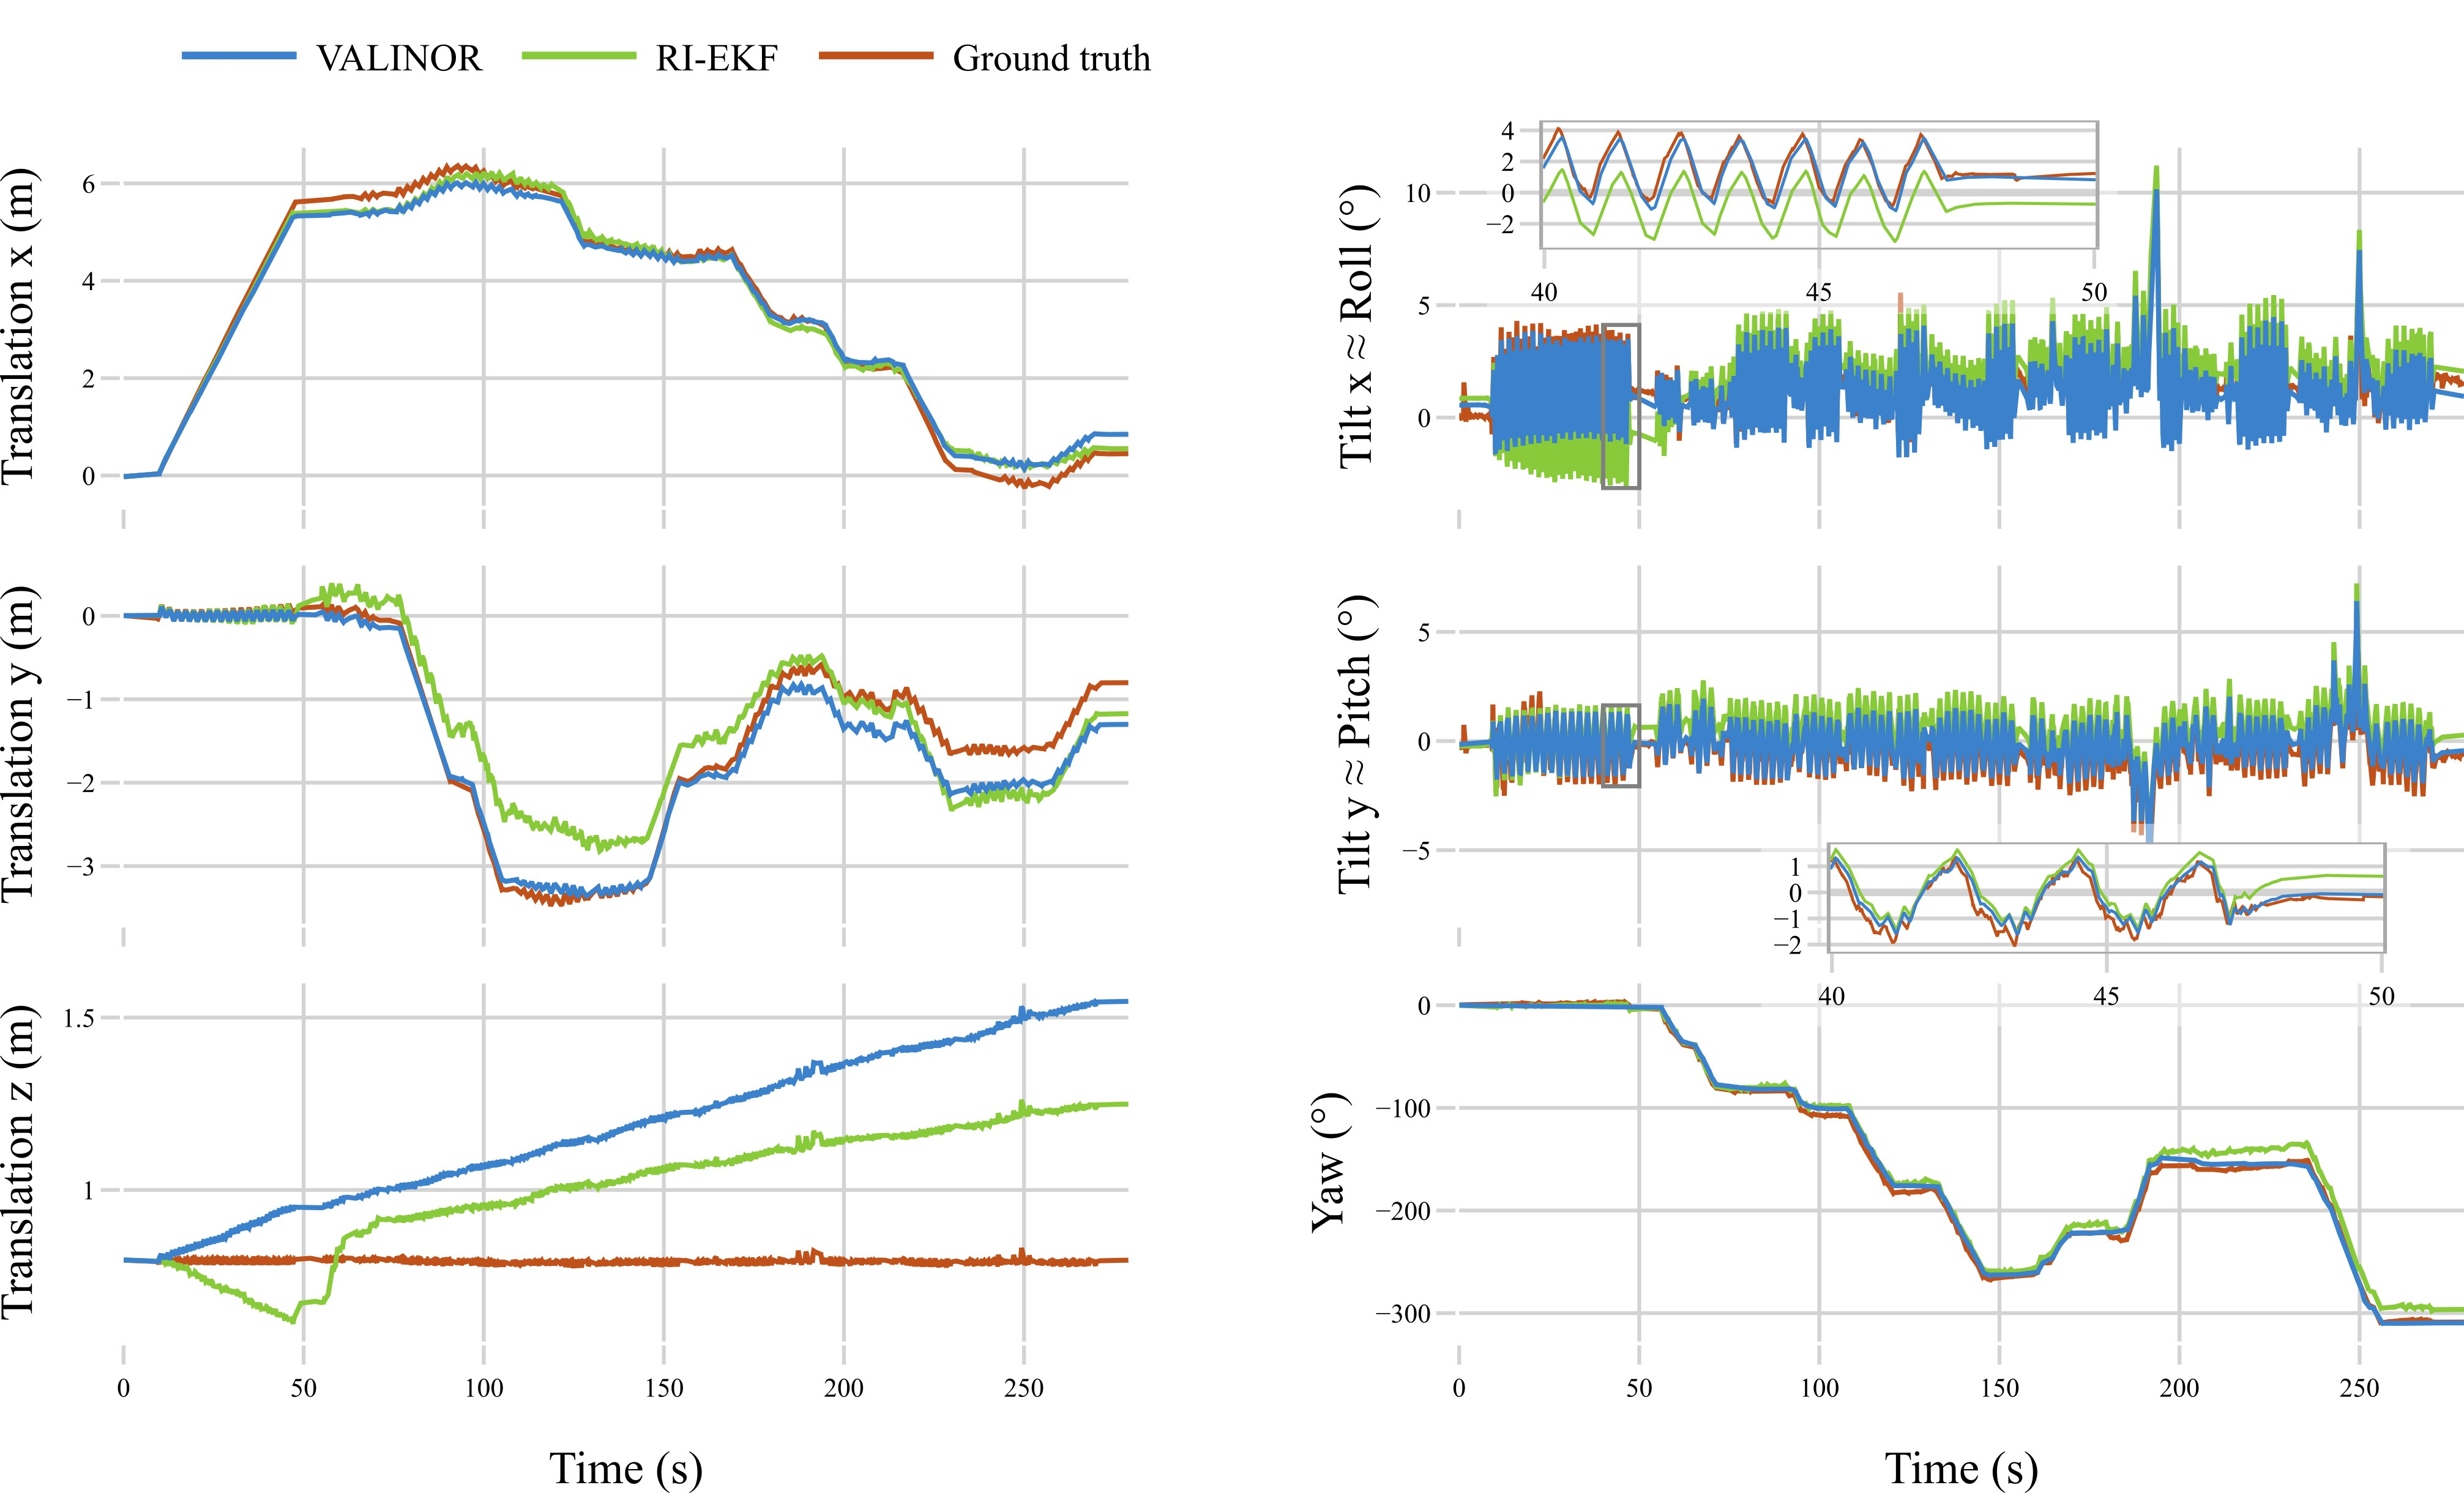
\includegraphics[width=0.89\textwidth]{pose.jpg} 
\vskip -0.5pc
\caption{Estimated and ground truth pose of RHP-Friends during the first walk on flat ground. Zoomed-in views are provided for the dense tilt plots, with a black rectangle indicating the corresponding area in the original plot.}\label{fig:pose_rhps1}
\end{center}
\vskip -1.5pc
\end{figure*}


\section{CONCLUSION}

In this paper, we proposed {\scshape Valinor}, a lightweight estimator for humanoid robots. By combining Leg odometry with the Tilt Observer, we could perform proprioceptive odometry whose accuracy rivalizes with the state-of-the-art method, while being over 7.5 times faster. Through this contribution, we aim to highlight the importance and the effectiveness of lightweight state estimation methods, especially in the current state of control for legged robots where computational efficiency is becoming a predominant challenge. We also seek to drive interest towards methods with mathematical guarantees, which we believe are essential for the safe industrial and societal deployment of legged robots. 

We note that by relying on Leg odometry and thus on the assumption of fixed contacts in the world, position and yaw estimation would drift from the actual ones in case of contact slippage~\cite{bloesch2013FusionLegKineAndImu}, as visible in Figure~\ref{fig:traj_friends}. Our method is particularly well suited to our intended use case of high-speed feedback for control in a local task space, but for tasks requiring minimal drift in absolute pose, methods using exteroceptive measurements~\cite{wisth2022vilens, fallon2018AccRobLocWalkRobotsImuVisLidar, Kuang2024TightlyCoupledLidarImuUwb}, although slower, would of course be more appropriate.
Further work would aim at reducing the sensitivity to slippage and other failure by improving the coupling between the Inertial and the Leg odometry, while preserving high computational efficiency. Other extensions could investigate the incorporation of other sensors into the framework.



\section*{DECLARATIONS}

\subsection*{Conflict of Interest }
The authors declare that there is no competing financial interest or personal relationship that could have appeared to influence the work reported in this paper.

\subsection*{Authors' Contributions}
Arnaud Demont and Mehdi Benallegue developed the proposed estimator's theoretical foundations. Abdelaziz Benallegue supervised the study and validated the theoretical framework. Arnaud Demont and Thomas Duvinage conducted the experiments. Arnaud Demont implemented the estimator and processed the experimental results. Arnaud Demont and Mehdi Benallegue wrote the manuscript in consultation with Thomas Duvinage and Abdelaziz Benallegue.

\subsection*{Funding }
This paper is based on results obtained from a project of Programs for Bridging the gap between R\&D and the IDeal society (society 5.0) and Generating Economic and social value (BRIDGE)/Practical Global Research in the AI x Robotics Services, implemented by the Cabinet Office, Government of Japan, and partially funded by the Japan Science and Technology Agency (JST) with the JST-Mirai Program, grant number JPMJMI21H4.


% \bibliographystyle{IJCAS}
% \bibliography{Bibliography}


\bibliographystyle{IEEEtran}
\bibliography{IEEEabrv, Bibliography}

\biography{Arnaud.jpg}{Arnaud Demont}{received the M.S. degree in mechanical engineering with a specialization in mechatronics and systems from the National Institute of Applied Sciences of Lyon, France, and a second M.S. degree in automation and robotics in intelligent systems from the University of  Technology of Compiègne, France, in 2021 and 2023 respectively. He is currently pursuing the PhD degree of the Université Paris-Saclay, France, within the CRNS-AIST Joint Robotics Laboratory in Tsukuba, Japan. His research interests include state estimation for legged robots, multi-sensor fusion, and mobile robot perception and autonomous navigation.
}

\biography{Mehdi.jpg}{Mehdi Benallegue}{holds an engineering degree from the National Institute of Computer Science (INI) in Algeria, obtained in 2007. He earned a master's degree from the University of Paris 7, France, in 2008, and a Ph.D. from the University of Montpellier 2, France, in 2011. His research took him to the Franco-Japanese Robotics Laboratory in Tsukuba, Japan, and to INRIA Grenoble, France. He also worked as a postdoctoral researcher at the Collège de France and at LAAS CNRS in Toulouse, France. Currently, he is a Research Associate with CNRS AIST Joint robotics Laboratory in Tsukuba, Japan. His research interests include robot estimation and control, legged locomotion, biomechanics, neuroscience, and computational geometry.
}

\biography{Thomas.jpg}{Thomas Duvinage}{received the M.S. degree in computer science with a specialization in robotics and computer vision from the University of Technology of Belfort-Montbéliard, France. He also holds a second M.S. degree in industrial and technology entrepreneurship from the same university. Since 2024, he has been serving as a CNRS delegate research engineer at the CNRS-AIST Joint Robotics Laboratory in Tsukuba, Japan. His work focuses on software integration for robotic systems, with research interests including robotics software architecture, system integration, and real-time robotic applications.
}

\biography{Aziz.jpg}{Prof. Abdelaziz Benallegue}{received the B.S. degree in electronics engineering from Algiers National Polytechnic School, Algeria in 1986 and both the M.S. and Ph.D. degrees in automatic control and robotics from University of Pierre and Marie Curie, Paris 6 (currently Sorbonne University), France in 1987 and 1991 respectively. He was Associate professor in Automatic Control and Robotics at the University Pierre et Marie Curie, Paris 6 (currently Sorbonne University) from 1992 to 2002. In September 2002, he joined the University of Versailles St Quentin as full Professor assigned. He was a CNRS delegate at JRL-AIST, Japan for three years, between 2016 and 2022. His research activities are mainly related to linear and non-linear estimation and control theory (adaptive control, robust control, neural learning control, observers, multi-sensor fusion, etc.) with applications in robotics (humanoid robots, aerial robots, manipulator robots, etc.).
}

\clearafterbiography
\relax 

\end{document}

